% \documentclass[a4paper,USenglish]{lipics-v2021}
\documentclass[a4paper,UKenglish,cleveref, autoref, thm-restate]{lipics-v2021}

\author{Orestis Alpos}{Common Prefix}{}{https://orcid.org/0000-0001-5477-3736}{}
\author{Bernardo David}{IT University of Copenhagen (ITU) \and Common Prefix}{}{https://orcid.org/0000-0002-1872-7799}{}
\author{Jakov Mitrovski}{Technical University of Munich \and Common Prefix}{}{}{}
\author{Odysseas Sofikitis}{Common Prefix \and \podtm network}{}{https://orcid.org/0009-0002-2154-0957}{}
\author{Dionysis Zindros}{Common Prefix \and \podtm network}{}{https://orcid.org/0000-0002-1978-594X}{}

\authorrunning{O. Alpos, B. David, J. Mitrovski, O. Sofikitis, and D. Zindros} %TODO mandatory. First: Use abbreviated first/middle names. Second (only in severe cases): Use first author plus 'et al.'

\Copyright{Orestis Alpos, Bernardo David, Jakov Mitrovski, Odysseas Sofikitis, and Dionysis Zindros} %TODO mandatory, please use full first names. LIPIcs license is "CC-BY";  http://creativecommons.org/licenses/by/3.0/

\ccsdesc{Security and privacy~Distributed systems security}
\ccsdesc{Computer systems organization~Dependable and fault-tolerant systems and networks}

\keywords{consensus, censorship resistance, accountability, auctions}

\relatedversiondetails[cite=DBLP:journals/corr/abs-2501-14931]{Full version}{https://arxiv.org/abs/2501.14931}

\EventEditors{Dariusz R. Kowalski}
\EventNoEds{1}
\EventLongTitle{39th International Symposium on Distributed Computing (DISC 2025)}
\EventShortTitle{DISC 2025}
\EventAcronym{DISC}
\EventYear{2025}
\EventDate{October 27--31, 2025}
\EventLocation{Berlin, Germany}
\EventLogo{}
\SeriesVolume{356}
\ArticleNo{5}

\usepackage{preamble}

\begin{document}

\title{
  \podtm: An Optimal-Latency, Censorship-Free, \\and Accountable Generalized Consensus Layer
}

\ccsdesc{Security and privacy~Distributed systems security}
\ccsdesc{Computer systems organization~Dependable and fault-tolerant systems and networks}

\keywords{consensus, censorship resistance, accountability, auctions}
% \author{Orestis Alpos}{Common Prefix}{}{}{}

% \author{Orestis Alpos\inst{1}\and
%   Bernardo David\inst{1,2}\and
%   Jakov Mitrovski\inst{1,3}\and\\
%   Odysseas Sofikitis\inst{1,4}\and
%   Dionysis Zindros\inst{1,4}
% }
% \institute{
%   Common Prefix\and
%   IT University of Copenhagen (ITU)\and
%   Technical University of Munich\and
%   \podtm network
% }


\maketitle

\begin{abstract}
This work addresses the inherent issues of high latency in blockchains and low scalability in traditional consensus protocols.
We present \podtm, a novel notion of consensus whose first priority is to achieve the physically-optimal latency of one round-trip, \textit{i.e.}, requiring only one network trip for writing a transaction and one for reading it.

To accomplish this, we first eliminate inter-replica communication. Instead, clients send transactions directly to all replicas, which independently process transactions and append them to local logs.
Replicas assigns a timestamp and a sequence number to each transaction in their logs, allowing clients to extract valuable metadata about the transactions and the system state. Later on, clients retrieve these logs and extract transactions (and associated metadata) from them.

Necessarily, this construction achieves weaker properties than a total-order broadcast protocol, due to existing lower bounds.
Our work models the primitive of \podtm and defines its security properties.
We then show \podtm-core, a protocol that satisfies properties such as transaction confirmation within $2\delta$, censorship resistance against Byzantine replicas, and accountability for safety violations. We show that single-shot auctions can be realized using the \podtm notion and observe that it is also sufficient for other popular applications.
%We show that a wide range of applications, such as payment systems, auctions, and decentralized data stores, can be based on a \podtm primitive.

%OLD
% Recent research shows many consensus applications do not require total order, even though they are usually realized on top of totally-ordered public ledgers. For example, for the double-spending problem in payments it suffices if a total order is only imposed within each user's set of transactions. For some applications not even this property is required. In a distributed auction, an auctioneer reads bids from the ledger at a prescribed \emph{deadline} and announces the winner according to the auction mechanism (\textit{e.g.}, highest bid wins). In this case, the order of bids does not matter, as long as the auctioneer cannot censor bids from parties who placed their bids \emph{before} the deadline.

% We present \podtm, a new distributed-systems notion, that achieves an \emph{evolving partial order} among transactions with \emph{past-perfection} guarantees.
% \emph{Evolving partial order} means that each transaction written to the system is assigned a non-fixed \emph{timestamp}, which may vary within an interval. Hence, transactions written sufficiently far from each other are ordered, while some transactions may appear as concurrent.
% \emph{Past perfection} guarantees that a party who reads the system sees \emph{all} transactions written up to a \emph{past-perfect round}, and, crucially, it cannot censor transactions by denying having seen them.

% %The efficiency gain that results from this simple observation is tremendous.
% The protocol we propose is latency-optimal and is executed by a number of \emph{replicas} and \emph{clients} in a way that %minimizes interaction among these parties. In particular,
% neither replicas nor clients communicate among each other. Clients read and write transactions by directly communicating with each replica. In this setting, replicas are accountable, \textit{i.e.}, replicas violating safety can be publicly identified. Building on this protocol, we realize auctions with accountable censorship resistance.

\end{abstract}

\section{Introduction}
Despite the widespread adoption of blockchains, a significant challenge remains unresolved: they are inherently slow. The latency from the moment a client submits a transaction to when it is confirmed in another client's view of the blockchain can be prohibitively long for certain applications. Notice that we define latency in terms of the blockchain \emph{liveness} property, referring to finalized, non-reversible outputs: once a transaction is received by a reader, it remains in the protocol's output permanently.
Moreover, we do not assume ``optimistic'' or ``happy path'' scenarios, where transactions might finalize faster under favorable conditions (such as having honest leaders or optimal network conditions).


Indeed, Nakamoto-style blockchain protocols require a large number of rounds in order to achieve consensus on a new block, even when considering the best known bounds~\cite{DBLP:conf/crypto/GaziRR23}. On the other hand, it is known that permissioned protocols for $n$ parties (out of which $t$ are corrupted) realizing traditional notions of broadcast and Byzantine agreement require at least $t+1$ rounds in the synchronous case~\cite{DBLP:journals/ipl/AguileraT99} and at least $2n/(n-t)$ rounds in the asynchronous case~\cite{DBLP:conf/focs/GarayKKO07}, even when allowing for digital signatures and probabilistic termination.


In a model where \emph{replicas} maintain the network, \emph{writers} submit transactions, and \emph{readers} read the network, the minimum latency is one network round trip, or $2\delta$, letting $\delta$ denote the actual network delay, as the information must travel from the writers to the replicas and then to the readers. More importantly, we want that any transaction from an honest writer appears in the output of honest readers within $2\delta$ time, regardless of the current value of $\delta$ and corrupted parties' actions.
In this context, we are motivated by the following question:

%\begin{center}
%	\emph{Can we perform payments -- and other tasks that blockchains are commonly used for -- in optimal latency?}
%\end{center}
\vspace{-2mm}
\begin{center}
	\emph{Can we realize tasks that blockchains are commonly used for with optimal latency?}
\end{center}
\vspace{-2mm}

We give a positive answer to this question with a protocol realizing \podtm, a new notion of consensus that trades off traditional agreement properties for optimal latency, while retaining sufficient security guarantees to realize important tasks (\textit{e.g.}, decentralized auctions).

\subsection{Our Contributions}
In order to motivate the notion of \podtm, we first introduce the architecture of our protocol, \podtm-core, which realizes this notion. To achieve the single-round-trip latency, our first key design decision is to eliminate inter-replica communication entirely. Instead, writers send their transactions directly to all replicas. Each replica maintains its own \emph{replica log}, processes incoming transactions independently, and transmits its log to readers on request. Readers then process these replica logs to extract transactions and relevant associated information. See Figure~\ref{fig:architecture} for a summary of the \podtm-core architecture.

\begin{figure}[ht]
    \centering
    \begin{minipage}{0.5\textwidth}
        \begin{center}
            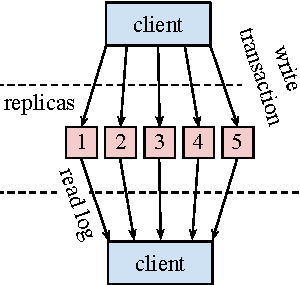
\includegraphics[width=0.55\textwidth]{figures/pod-architecture.pdf}
        \end{center}
    \end{minipage}%
    \hfill
    \begin{minipage}{0.5\textwidth}
        \caption{\podtm-core's simple architecture. A writing client (top) sends a transaction to all replicas (middle). Each replica appends it to its own log and transmits it to the reading client (bottom).}
        \label{fig:architecture}
    \end{minipage}
\end{figure}

This design raises two important questions. First, what meaningful information can readers derive from replica logs when replicas operate in isolation? Second, given that in two rounds even randomized authenticated broadcast is proven impossible~\cite{DBLP:conf/focs/GarayKKO07}, what capabilities can this -- necessarily weaker -- primitive offer? We demonstrate that, by incorporating simple mechanisms, such as assigning timestamps and sequence numbers to transactions, replicas can enable readers to extract valuable information beyond mere low-latency guarantees. Furthermore, we show how the properties of \podtm can enable various applications, including auctions (as shown in \Cref{sec:auctions}).
Specifically, a secure \podtm delivers the following guarantees (formally defined in \Cref{sec:pod-model}):
\begin{itemize}
    \item Transaction confirmation within $2\delta$, with each transaction assigned a \emph{\confirmed round}: we say that the transaction becomes \emph{confirmed} at the time indicated by the \emph{confirmed round}.
    \item Censorship resistance when facing up to $\beta$ Byzantine and $\gamma$ omission-faulty replicas, ensuring all confirmed transactions appear in every honest reader's output.
    \item A \emph{past-perfect round} can be computed by readers, such that the reader is guaranteed to have received all transactions that are or will be confirmed prior to this round, even though not all transactions are strictly ordered.
    \item Accountability for all safety violations, \textit{i.e.}, if any safety property is violated, at least $\beta + 1$ replicas can be identified as misbehaving.
\end{itemize}

In particular, our Protocol \podtm-core, presented in \Cref{sec:pod-core-const}, realizes the notion of \podtm with the properties above, supporting a continuum of two adversarial models: up to \beta Byzantine replicas and up to \gamma omission-faulty replicas, out of a total of $n > 5 \beta + 3 \gamma$ replicas.
Protocol \podtm-core requires no expensive cryptographic primitives or setup beyond digital signatures and a PKI registering replicas' public keys. We showcase \podtm-core's efficiency by means of experiments with a prototype implementation presented in \Cref{sec:evaluation}. Our experiments show that even with 1000 replicas distributed around the world, the latency achieved by our protocol is just under double (resp. about 5 times) the round-trip time between writer and reader clients with security against omission-faulty (resp. Byzantine) replicas.


\subsection{Technical Overview}
We consider that time proceeds in \emph{rounds}, and that parties (replicas and clients) know the current round, so we can express \emph{timestamps} in terms of rounds. The output of \podtm associates each transaction $\tx$ with timestamp values $\rmin \geq 0$ (minimum round), $\rmax \leq \infty$ (maximum round) and $\rconf$ (\emph{confirmed round}). We call these values the \emph{trace} of \tx, and they evolve over time.
Initially we have $\rconf=\perp$ but later we get $\rconf \neq \perp$, when a transaction is \emph{confirmed}. The protocol guarantees \emph{confirmation within $u$ rounds}, meaning that, at most $u$ rounds after $\tx$ was written, every party who reads the \podtm will see $\tx$ as confirmed with some $\rconf \neq \perp$.
The protocol also guarantees that $\rmin \leq \rconf \leq \rmax$, a property we call \emph{confirmation bounds}:
while each party reads different values $\rmin,\rmax,\rconf$ for the same $\tx$, \podtm guarantees that values read by different parties stay within these limits.

When clients \emph{read} the \podtm, they obtain a $\podtm$ data structure $\Pod = (\txSet, \rperf)$, where $\txSet$ is the set of transactions and their traces and $\rperf$ is a \emph{past-perfect} round. The \emph{past-perfection} safety property guarantees that
%if a transaction $\tx$ did not appear in $\txSet$, then no other party will ever read $\tx$ with confirmed round $\rconf'$ such that $\rconf' < \rperf$. This guarantees that,
\txSet contains \emph{all} transactions that every other honest party will ever read with a confirmed round smaller than $\rperf$.  A \podtm also guarantees \emph{past-perfection within $w$}, meaning that $\rperf$ is at most $w$ rounds in the past.

% For each transaction $\tx$ in \txSet, the reader obtains associated timestamps $\rmin,\allowbreak \rmax, \rconf$ and auxiliary data $\txcert$, which may evolve. The protocol guarantees \emph{confirmation within $u$ rounds}, meaning that, at most $u$ rounds after $\tx$ was written, every party who reads the \podtm will see $\tx$ as confirmed with some $\rconf \neq \perp$.
% Moreover, \podtm guarantees \emph{confirmation bounds}, ensuring that
% % if a party reads $\tx$ with minimum round $\rmin$ and maximum round $\rmax$, for every other party who reads $\tx$ with $\rconf' \neq \perp$, it holds that $\rmin \leq \rconf' \leq \rmax$. This means that
% the values \rmin and \rmax for $\tx$, read by an honest party, determine the range of the \rconf value for $\tx$ that can ever be read by another honest party,
% i.e., $\rmin \leq \rconf \leq \rmax$.

In summary, \podtm provides \emph{past-perfection} and \emph{confirmation bounds} as safety properties, ensuring parties cannot be blindsided by transactions suddenly appearing as confirmed too far in the past, and that the different (and continuously changing) transaction timestamps stay in a certain range. The liveness properties of \emph{confirmation within $u$} and \emph{past-perfection within $w$} ensure that new transactions get confirmed within a bounded delay, and that each party's past-perfect round must be constantly progressing.

Besides introducing the notion of \podtm, we present protocol \podtm-core, which realizes this notion while requiring minimal interaction among parties and achieving optimal latency, \textit{i.e.}, optimal parameters $u=2\delta$ and $w=\delta$, where $\delta$ is the current network delay (not a delay upper bound, which we assume to be unknown).
% Our construction relies on a set of $n$ \emph{replicas} to maintain a \podtm data structure, which can be read by an unknown number of clients.
The only communication is between each client and the replicas.
% Moreover, \podtm-core can use the auxiliary data $\ppcert,\txcert$ to publicly identify misbehaving replicas and keep them accountable.
Writing a transaction $\tx$ to \podtm-core only requires clients to send $\tx$ to the replicas, who each assign a timestamp $\tsp$ (their current time) and a \emph{sequence number} \sn to $\tx$ and return a signature on $(\tx,\tsp, \sn)$. When reading the \podtm, the client simply requests each replica's log of transactions, validates the responses, and determines $\rmin$, $\rmax$, and \rconf from the received timestamps.
% If the client receives responses from enough replicas, $\rconf$ is determined by taking the median of the timestamps received from these replicas.
% If a replica provides conflicting timestamps $\tsp\neq \tsp'$ for the same $\tx$ to one or more clients, the replica's signatures publicly proves cheating.
Protocol \podtm-core supports a continuum of mixed adversarial models, tolerating up to \beta Byzantine \emph{and} at the same time up to \gamma additional omission-faulty replicas.
% However, although we prove our results for executions with only Byzantine and only omission faults, we conjecture that Protocol \podtm-core realizes the \podtm notion for a continuum between these two cases. We leave the security analysis of our protocol under a continuum of mixed Byzantine and omission faults to the full version of this work.

%\todo{A paragraph on feed-layers ad decentralized social applications}


\subsection{Related work}\label{app:related}

% \dotparagraph{Reducing latency}
Many previous works have lowered the latency of ordering transactions.
HotStuff~\cite{DBLP:conf/podc/YinMRGA19} uses three rounds of all-to-leader and leader-to-all communication pattern, which results in a latency (measuring from the moment a client submits a transaction until in appears in the output of honest replicas) of $8\delta$ in the happy path.
Jolteon~\cite{DBLP:conf/fc/GelashviliKSSX22}, Ditto~\cite{DBLP:conf/fc/GelashviliKSSX22}, and HotStuff-2~\cite{DBLP:journals/iacr/MalkhiN23} are two-round versions of HotStuff with end-to-end latency of $5\delta$.
MoonShot~\cite{DBLP:journals/corr/abs-2401-01791} allows leaders to send a new proposal every $\delta$ time, before receiving enough votes for the previous one, but still achieves an end-to-end latency of $5\delta$.
In the ``DAG-based'' line of word, Tusk~\cite{DBLP:conf/eurosys/DanezisKSS22} achieves and end-to-end latency of $7\delta$,
the partially-synchronous version of BullShark~\cite{DBLP:journals/corr/abs-2209-05633} an end-to-end latency of $5\delta$,
and Mysticeti~\cite{DBLP:journals/corr/abs-2310-14821} an end-to-end latency of $4\delta$.
All these protocols aim at total-order properties and have their lower latency is inherently restricted by lower bounds, whereas \podtm starts from the single-round-trip latency requirement and explores the properties that can be achieved.

The redundancy of consensus for implementing payment systems has been recognized by previous works~\cite{DBLP:journals/dc/GuerraouiKMPS22,DBLP:journals/corr/abs-1909-10926,DBLP:conf/dsn/CollinsGKKMPPST20,DBLP:conf/aft/BaudetDS20}.
The insight is that total transaction order is not required in the case that each account is controlled by one client.
Instead, a partial order is sufficient, ensuring that, if transactions $\tx_1$ and $\tx_2$ are created by the same client, then every party outputs them in the same order.
This requirement was first formalized by Guerraoui~\etal~\cite{DBLP:journals/dc/GuerraouiKMPS22} as the \emph{source-order property}.
The constructions of Guerraoui~\etal~\cite{DBLP:journals/dc/GuerraouiKMPS22} and FastPay~\cite{DBLP:conf/aft/BaudetDS20} require clients to maintain sequence numbers.
ABC~\cite{DBLP:journals/corr/abs-1909-10926} requires clients to reference all previous transaction in a DAG (including its own last transaction).
% , and, in case of transactions spending the same output, by having replicas sign only one of them.
Cheating clients might lose liveness~\cite{DBLP:conf/aft/BaudetDS20,DBLP:journals/dc/GuerraouiKMPS22,DBLP:journals/corr/abs-1909-10926}, but equivocating is not possible.
To the best of our knowledge, previous work in the consensusless literature has not considered or achieved a property like our \emph{past-perfection}, which we show sufficient for implementing auctions.
\section{Preliminaries}

% \dotparagraph{Notation}
\textbf{Notation:} We denote by \BN the set of natural numbers including $0$.
Letting $L$ be a bounded sequence, we denote by $L[i]$ the $i^\text{th}$ element (starting from $0$),
and by $|L|$ its length.
Negative indices address elements from the end, so $L[-i]$ is the $i^\text{th}$ element from
the end, and $L[-1]$ in particular is the last.
%We use $L[i{:}j]$ to denote the subarray of $L$
% consisting of the elements indexed from $i$ (inclusive) to $j$ (exclusive).
The notation $L[i{:}]$ means the
subarray of $L$ from $i$ onwards, while $L[{:}j]$ means the subsequence of $L$ up to (but not including) $j$.
We denote an empty sequence by $[\,]$.
We denote the concatenation of sequences $L_1$ and $L_2$ by $L_1 \concat L_2$.

\textbf{Pseudocode notation:} Command `\textbf{require} $P$' causes a function to terminate immediately and return $\false$ if $P$ evaluates to $\false$.
Notation `\textbf{upon} $e$' causes a block of code to be executed when event $e$ occurs.
Notations `$\msg{MSG}{} \leftarrow p$' and `$\msg{MSG}{} \rightarrow p$' denote receiving and sending a message $MSG$ from and to party $p$, respectively.
Finally, $x: a \in A \rightarrow b \in B$ denotes that variable $x$ is a map from elements of type $A$ to elements of type $B$. When obvious from the context, we do not explicitly write the types $A$ or $B$.
For a map $x$, the operations $x.\opKeys$ and $x.\opValues$ return all keys and all values in $x$, respectively.
With $\emptyset$ we denote an empty map.
% \subsection{Execution Model}
\label{sec:system}

\textbf{Parties:}
We consider $n$ \emph{replicas} $\replicas=\{\replicas_1,\ldots,\replicas_n\}$ and an unknown number of \emph{clients}. Parties are \emph{stateful}, \textit{i.e.}, store \emph{state} between executions of different algorithms.
We assume that replicas are known to all parties and register their public keys (for which they have corresponding secret keys) in a Public Key Infrastructure (PKI). Clients do not register keys in the PKI.
% \vspace{-3mm}

\textbf{Adversarial model:}
We call a party (replica or client) \emph{honest}, if it follows the protocol, and \emph{malicious} otherwise.
% Our constructions assume limits on \alpha and \beta, but make no honesty assumptions on clients.
We assume \emph{static corruptions},  \textit{i.e.}, the set of malicious replicas is decided before the execution starts and remains constant.
This work uses a combination of two adversarial models, the \emph{Byzantine} and the \emph{omission} models.
In the \emph{Byzantine} model, corrupted replicas are malicious and may deviate arbitrarily from the protocol. The adversary has access to the internal state and secret keys of all corrupted parties. We denote by $\beta \in \BN$ the  number of Byzantine replicas in an execution.
The Byzantine adversary is modelled as a probabilistic polynomial time overarching entity that is invoked in the stead of every corrupted party.
That is, whenever the turn of a corrupted party comes to be invoked by the environment, the adversary is invoked instead.
In the \emph{omission} model, corrupted replicas may only deviate from the protocol by dropping messages that they were supposed to send, but follow the protocol otherwise. Observe that this includes crash faults, where replicas crash (\textit{i.e.} stop execution) and remain crashed until the end of the execution of an algorithm. We denote by $\gamma \in \BN$ the number of omission-faulty replicas in an execution.

% \oa{We allow \emph{dynamic corruptions}, i.e., the set of malicious replicas can differ in each round, as long as not larger than \beta.}

%\vspace{-3mm}
%\dotparagraph{Stateful clients} A stateful client is a party who stores \emph{state} (\textit{i.e.}, data) between executions of different algorithms.
% \vspace{-3mm}

\textbf{Modeling time:}
We assume that time proceeds in discrete \emph{rounds}, and parties have clocks allowing them to determine the current round.
For simplicity, our analysis will assume \emph{synchronized clocks}.
Notice that although we assume synchronized clocks as a setup, clock synchronization can be achieved in partially synchronous networks~\cite{psync} using existing techniques~\cite{clockoverview}, also in the case where replicas gradually join the network~\cite{bootclocksync}.
% We denote by $\tzero$ the round at which the execution starts.
By \emph{timestamp} we refer to a round number assigned to some event.

\textbf{Modeling network:}
We denote by $\delta \in \CN$ the actual delay (measured in number of rounds) it takes to deliver a message between two honest parties,
a number which is \emph{finite} but \emph{unknown} to all parties.
We denote by $\Delta \in \CN$ an upper bound on this delay, \textit{i.e.}, $\delta \leq \Delta$, which is also \emph{finite}.
In the \emph{synchronous} model, $\Delta$ is \emph{known} to all parties.
% (namely, the honest code is parametrized by $\Delta$).
In the \emph{partially synchronous} model~\cite{psync}, $\Delta$ is \emph{unknown} but still finite, \textit{i.e.}, all messages are eventually delivered.
%The environment is constrained to deliver all honest network messages within $\delta$. Namely, for each message $m$ sent
%by an honest party at round $r$, the environment observes and remembers the inboxes (decided by the adversary)
%of all honest parties during rounds $r + 1, \ldots, r + \delta$. If none of these inboxes contains $m$, the environment
%appends $m$ to the network inbox of the recieving party prior to invoking it at round $r + \delta$, thereby forcing the
%inclusion of this message.
% In this work, we present a general protocol, which we then analyze in the \emph{synchronous} and in the \emph{asynchronous} models, providing different guarantees in each world.
% We now define responsive protocols, which is the case of our main protocol \podtm-core.
A protocol is called \emph{responsive} if it does not rely on knowledge of $\Delta$ and its liveness guarantees depend only on the actual network delay $\delta$.
%this is very fluffy, we should make it precise for the DISC submission.

% \subsection{Cryptographic primitives}
\dotparagraph{Digital signatures} We assume that replicas (and auctioneers in \bidsettm-core) authenticate their messages with digital signatures. A digital signature scheme consists of the following three algorithms, satisfying the EUF-CMA security~\cite{GMR88}:
(1) $\textsl{KeyGen}(1^{\kappa})$:
The key generation algorithm takes as input a security parameter $\kappa$ and outputs a secret key $\sk$ and a public key $\pk$.
(2) $\opSign{\sk, m} \rightarrow \sig$:
The signing algorithm takes as input a private key
\sk and a message $m \in \zo^*$ and returns a signature $\sig$.
(3)$\opVerify{\pk, m, \sig} \rightarrow b \in \zo$:
The verification algorithm takes as input a public
key $\pk$, a message $m$, and a signature $\sig$, and outputs a bit $b\in \zo$.
We say \sig is a \emph{valid} signature on $m$ with respect to \pk if $\opVerify{pk, m, \sig} = 1$.





\dotparagraph{Accountable safety}
\label{sec:accountable-safety}
Taking a similar approach as Neu, Tas, and Tse~\cite[Def. 4]{FC:NeuTasTse22}, we define \emph{accountable safety} through an \emph{identification function}.

\begin{definition}[Transcript and partial transcript]
    We define as \emph{transcript} the set of all network messages sent by all parties in an execution of a protocol.
    A \emph{partial transcript} is a subset of a transcript.
\end{definition}

\begin{definition}[\beta-Accountable safety]\label{def:accountable-safety}
    A protocol satisfies \emph{accountable safety} with \emph{resilience} \beta if its interface contains a function $\identify{\tran} \rightarrow \cheaters$,
    which takes as input a partial transcript $\tran$ and outputs a set of replicas $\cheaters \subset \replicas$, such that the
    following conditions hold except with negligible probability.
    \begin{description}
        \item[Correctness:] If safety is violated, then there exists a partial transcript \tran, such that $\identify{\tran} \rightarrow \cheaters$ and $|\cheaters| > \beta$.
        \item[No-framing:] For any partial transcript \tran produced during an execution of the protocol, the output of $\identify{\tran}$ does not contain honest replicas.
    \end{description}
\end{definition}

\begin{remark}
    For simplicity, we have defined the transcript based on messages sent by \emph{all} replicas.
    We can also define a \emph{local transcript} as the set of messages observed by a single party.
    As will become evident from the implementation of \identify{}, in practice, adversarial behavior can be identified from the local transcripts of a single party or  of a pair of parties.
    %This optimization can be used in the implementation of a protocol.
\end{remark}
\section{Modeling \podtm} \label{sec:pod-model}
In this section, we introduce the notion of a \podtm, a distributed protocol where clients can \emph{read} and \emph{write} transactions.
We first define the basic data structures of a \podtm protocol.

\begin{definition}[Transaction trace and trace set]
    The \emph{transaction trace} of a transaction $\tx \in \zo^*$ is a tuple containing the values $(\tx, \rmin, \rmax, \rconf)$, which change during the execution of a \podtm protocol.
    We call $\rmin \in \BN$ the \emph{minimum round}, $\rmax \in \BN \cup \{\infty\}$ the \emph{maximum round},
    $\rconf \in \BN \cup \{\bot\}$ the \emph{\confirmed round}.
    We denote by $\rmax=\infty$ an unbounded maximum round and by $\rconf=\bot$ an undefined \confirmed round.
    We also denote these values as $\tx.\rmin, \tx.\rmax$, and $\tx.\rconf$.
    A \emph{trace set} $\txSet$ is a set of transaction traces $\{(\tx, \rmin, \rmax, \rconf) \mid \tx \in \zo^*\}$.
\end{definition}

\begin{definition}[Confirmed transaction]
    A transaction with confirmed round \rconf is called \emph{\confirmed} if $\rconf \neq \bot$, and \emph{unconfirmed} otherwise.
\end{definition}

% \begin{definition}[Trace set]
% A \emph{trace set} $\txSet$ is a set of traces $(\tx, \rmin, \rmax, \rconf)$. We say that a transaction $\tx$ \emph{appears} in $\txSet$ when $\exists (\tx, \rmin, \rmax, \rconf) \in \txSet$, otherwise we say that a transaction $\tx$ \emph{does not appear} in $\txSet$.
% \end{definition}


\begin{definition}[Pod data structure]
    A \emph{pod data structure} $\Pod$ is a tuple $(\txSet, \rperf)$, where \txSet is a trace set and \rperf is a round number called the \emph{past-perfect round}.
\end{definition}
We denote the components of a pod data structure as $\Pod.\txSet$ and $\Pod.\rperf$.
We write $\tx \in \Pod.\txSet$ if an entry $(\tx, \cdot, \cdot, \cdot)$ exists in $\Pod.\txSet$.
We remark that transactions in \txSet may be \confirmed on unconfirmed. Moreover, \rperf will be used to define a completeness property on \txSet (the \emph{past-perfection} property of \podtm).

\begin{definition}[Auxiliary data]
    We associate with a pod data structure $\Pod$ some auxiliary data \cert, which will be used to validate \Pod.
    The exact implementation of \cert is irrelevant for the definition of \podtm;
    however, it is helpful to mention that in \podtm-core it will be a tuple $\cert = (\ppcert, \alltxcert)$,
    where $\ppcert$ will be a \emph{past-perfection certificate} and \alltxcert a map from each transaction \tx in $\Pod.\txSet$ to a \emph{transaction certificate} \txcert for \tx.
    Both contain digital signatures.
\end{definition}

%We now define the \podtm protocol interface and associated concepts.
\begin{definition}[Interface of a \podtm]\label{def:podinterface}
A \podtm protocol has the following interface.
\begin{itemize}
    \item $\opwrite{\tx}$:
    % \item $\opwrite{\tx} \returns (\rmin, \rmax, \rconf, \txcert)$:
    It writes a transaction \tx to the \podtm.

    \item $\opreadall{} \returns (\Pod, \cert)$:
    It outputs a pod data structure $\Pod = (\txSet, \rperf)$ and auxiliary data \cert.
    % The second output is called an \emph{equivocation-evidence pod} and can be either $\bot$ or $\tilde{\Pod} = (\tilde{\txSet}, \tilde{\rperf}, \tilde{\ppcert})$.
\end{itemize}
\end{definition}
We say that a client \emph{reads the} \podtm when it calls \opread{}.
If $\tx$ appears in $\txSet$,
%$(\tx, \rmin, \rmax, \rconf, \txcert) \in \txSet$
 we say that the client \emph{observes} \tx and, if $\tx.\rconf \neq \bot$, we say that the client \emph{observes \tx as \confirmed}.

\begin{definition}[Validity function]
    Apart from its interface functions,
    a pod protocol also specifies a computable, deterministic, and non-interactive function \opValid{\Pod, \cert} that takes as input a pod data structure $\Pod$ and auxiliary data $\cert$ and outputs a boolean value. We say that a pod data structure $\Pod$ is \emph{valid} if $\opValid{\Pod, \cert} = \true$.
\end{definition}


% \begin{definition}[Past-perfect round]
% 	Given a set \txSet obtained by an honest client who reads the pod, a round \rperf is \emph{past-perfect} if,
% 	for any transaction $\tx$ that does not appear in $ \txSet$, no honest client will ever observe \tx as confirmed with $\tx.\rconf < \rperf$.
% \end{definition}

\begin{definition}[View of the \podtm]
    We call \emph{view of the} \podtm and denote by \podView{\client}{\round} the data structure returned by \opreadall{}, where \opreadall{} is invoked by client \client and the output is produced at round \round.
    We remark that \round denotes the round when \opreadall{} outputs, as the client may have invoked it at an earlier round.
    % We denote the components of a view as $\podView{\client}{\round}=(\podView{\client}{\round}.\txSet,
    % \podView{\client}{\round}.\rperf)$.
    % We write $\tx \in \podView{\client}{\round}$ if $\tx$ appears in $\podView{\client}{\round}.\txSet$.
\end{definition}

We now introduce the basic definition of a \emph{secure} \podtm protocol, as well as some additional properties (\emph{timeliness} and \emph{monotonicity}) that it may satisfy.

\begin{definition}[Secure \podtm]\label{def:podsec}
A protocol is a \emph{secure} \podtm if it implements the \podtm interface of Definition~\ref{def:podinterface} and specifies a validity function \opValid{}, such that the following properties hold.
\begin{description}
    \item[(Liveness) Completeness:]
    Honest clients always output a valid pod data structure.
    That is, if \opread{} returns $(\Pod, \cert)$ to an honest client, then $\opValid{\Pod, \cert} = \true$.

    \item[(Liveness) Confirmation within \parConf:]
	Transactions of honest clients become \confirmed after at most \parConf rounds.
	Formally, if an honest client $\client$ writes a transaction \tx at round \round,
    then for any honest client $\client'$ (including $\client=\client'$) it holds that $\tx \in \podView{\client'}{\round + \parConf}$ and $\tx.\rconf \neq \bot$.


	\item[(Liveness) Past-perfection within \parPerf:]
	Rounds become past-perfect after at most $\parPerf$ rounds.
	Formally,
    for any honest client \client and round $\round \geq \parPerf$, it holds that $\podView{c}{\round}.\rperf \geq \round - \parPerf$.
    % for any valid pod \Pod obtained at round \round, it holds that $\Pod.\rperf \geq \round - \parPerf$.

	\item[(Safety) Past-perfection:]
    A valid pod \Pod contains all transactions that may ever obtain a \confirmed round smaller than $\Pod.\rperf$. Formally,
	the adversary cannot output $(\Pod_1, \cert_1)$ and $(\Pod_2, \cert_2)$ to the network, such that $\opValid{\Pod_1, \cert_1} \land \opValid{\Pod_2, \cert_2}$ and there exists a transaction $\tx$ such that $(\tx, \rmin^1, \rmax^1, \rconf^1) \not\in \Pod_1.\txSet$ and $(\tx, \rmin^2, \rmax^2, \rconf^2) \in \Pod_2.\txSet$ and $\rconf^2 \neq \bot$ and $\rconf^2 < \Pod_1.\rperf$.

	\item[(Safety) Confirmation bounds:]
    \sloppy{
    The values $\rmin$ and $\rmax$ bound the \confirmed round that a transaction may ever obtain. Formally,
    the adversary cannot output $(\Pod_1, \cert_1)$ and $(\Pod_2, \cert_2)$ to the network, such that $\opValid{\Pod_1, \cert_1} \land \opValid{\Pod_2, \cert_2}$ and there exists a transaction $\tx$ such that $(\tx, \rmin^1, \rmax^1, \rconf^1) \in \Pod_1.\txSet$ and $(\tx, \rmin^2, \rmax^2, \rconf^2) \in \Pod_2.\txSet$ and $\rmin^1 > \rconf^2$ or $\rmax^1 < \rconf^2$.
    }

    % \oa{\item[(Safety) Censorship resistance:]}
	% If the adversary makes progress (outputs some past-perfect round), then it must output all transactions confirmed up that past perfect round, minus some propagation period of $X$.
	% Formally, there is a parameter $X$ such that,
    % if the adversary outputs $(\Pod, \cert)$ to the network with $\opValid{\Pod, \cert}$, then \Pod contains all transaction with confirmed round $\rconf \geq \Pod.\rperf - X$.
    % \oa{This is not exactly true, the adversary may see a transaction with $\alpha - \beta$ votes. It would be true if the confirmation threshold was $\alpha  - \beta$. What is its connection with the past-perfection safety property?}
\end{description}
\end{definition}


%The \emph{confirmation within \parConf} property gives us that, if an honest client writes a transaction \tx, then \tx will obtain $\rconf \neq \bot$ within \parConf rounds, but it does not tell us \emph{what} that \rconf will be.
%Similarly,
The \emph{confirmation bounds} property gives $\rmin^1 \leq \rconf^2 \leq \rmax^1$, for $\rmin^1, \rmax^1, \rconf^2$ computed by honest clients, but it does not guarantee anything about the values of $\rmin^1$ and $\rmax^1$ (for example, it could trivially be $\rmin^1=0$ and $\rmax^1=\infty$).
To this purpose we define an additional property of \podtm, called \emph{timeliness}.
% , which can be satisfied along with the standard safety and liveness properties of \podtm.
Previous work has observed a similar property as orthogonal to safety and liveness~\cite{EPRINT:TziSriZin23}.

\begin{definition}[\podtm \parTemp-timeliness for honest transactions]\label{def:pod-timely}
    A \podtm protocol is \emph{\parTemp-timely} if it is a secure \podtm, as per Definition~\ref{def:podsec}, and for any honest clients $\client_1,\client_2$, if $\client_1$ writes transaction \tx in round $\round$ and $\client_2$ has view $\podView{\client_2}{\round'}$ in round $\round'$, such that $(\tx, \rmin, \rmax, \rconf) \in \podView{\client_2}{\round'}.\txSet$, then:\\
    % (observe that, from the \emph{confirmation within \parConf} property, \tx will become confirmed):
    % \begin{enumerate}
        (1) $\rconf \in (\round, \round + \parTemp]$;
        (2) $\rmax \in (\round, \round + \parTemp]$;
        (3) $\rmax - \rmin < \parTemp$, implying $\rmin \neq 0$ and $\rmax \neq \infty$.
    % \end{enumerate}
\end{definition}


Moreover, a \podtm protocol allows \rmin, \rmax, \rconf to change during an execution -- for example, clients in construction \podtm-core will update them when they receive votes from replicas.
In the full version of this paper~\cite[Appendix A]{DBLP:journals/corr/abs-2501-14931} we define \emph{monotonicity} properties that impose restrictions on how these values evolve.

We conclude this section with some visual examples in Figures \ref{fig:temperature} and \ref{fig:example-output}.
% \begin{figure}[h]
%     \centering
%     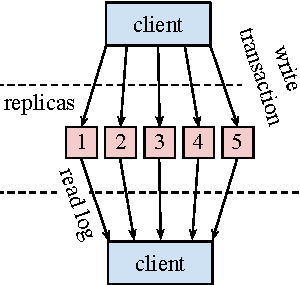
\includegraphics[width=0.35\textwidth]{figures/pod-architecture.pdf}
%     \caption{\todo{Add figure} }
%     \label{fig:example-output}
% \end{figure}


\begin{figure}[ht]
    \begin{minipage}[b]{.48\textwidth}
    \centering
    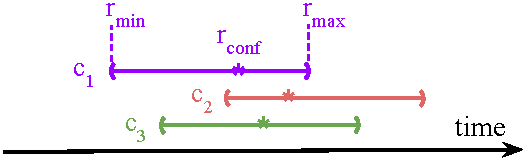
\includegraphics[width=1\textwidth]{figures/pod-temperature.pdf}
    \caption{The same transaction in the view of three different pod clients. Each client assigns it a minimum round \rmin and a maximum round \rmax. If it gets confirmed, the confirmation round \rconf will be
     between these two values. The \rconf that each client locally computes respects the bounds of each other client.}
     \label{fig:temperature}
    \end{minipage}
    \hfill
    \begin{minipage}[b]{.49\textwidth}
    \centering
    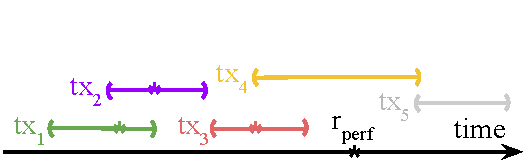
\includegraphics[width=1\textwidth]{figures/pod-example.pdf}
    \caption{A possible view of a single pod client.
    Transactions $\tx_1, \tx_2, \tx_3$ are confirmed, $\tx_4$ is not yet confirmed.
    A client also derives a past-perfect round $\rperf$. No transaction other than $\tx_1, \tx_2, \tx_3, \tx_4$ may  obtain $\rconf \leq \rperf$. There may exist $\tx_5$ for which the client has not received votes, but $\tx_5$ cannot obtain $\rconf \leq \rperf$.
    % Transactions written concurrently, or close to each other, such as $\tx_3$ and $\tx_4$, may not be totally ordered. Transactions written by malicious clients, such as $\tx_5$ may not become confirmed.
    }
    \label{fig:example-output}
    \end{minipage}
\end{figure}



% \subsection {Properties recap}
% This is for us. It summarizes the aforementioned properties and shows which algorithms satisfy them.
% \begin{center}
%     \begin{tabular}{ |l|c|c||c|c|c| }
%         \hline
%                                                                & \multicolumn{2}{c||}{streaming} & \multicolumn{2}{c|}{streaming+gossip}\\
%         \hline
%                                                                & sync  & async  &sync & async \\
%         Confirmation                                           & O& O& O& O\\
%         Pp liveness                                            & O& O& O& O\\
%         Common subset                                          & X& X& O& O\\
%         Common subset for honest tx                            & O& O& O& O\\
%         Conf. stickiness                                       & O& O& O& O\\
%         Correctness of assoc. values                           & O& O& O& O\\
%         Pp correctness                                         & O& O& O& O\\
%         Pp stickiness                                          & O& O& O& O\\
%         \hline
%     \end{tabular}
%     \end{center}

\section{Protocol \podtm-core}\label{sec:pod-core-const}
% The construction employs the \emph{client gossip} technique. It could be the case that
% clients perform read operations on the replicas and observe that some of them miss some data, such as client transactions.
% Client gossip consists in having clients re-broadcast these missing transactions.
% This technique ensures the client that a round becomes past perfect,
% hence the client has a finalized view of the system: a transaction that was re-broadcast will
% eventually reach all honest replicas, hence it cannot get removed from the system in the future.
% \oa{TODO: Mention that we can use client gossip, gossiping, or relayers to achieve totality. We denote by $u$ the (average) time it takes
% in synchrony for a transaction to reach all replicas. For example, $u = 2 \Delta$ using client gossip or relayers.}

Before we present protocol \podtm-core, we define basic concepts and structures.

\begin{definition}[Vote]
    A \emph{vote} is a tuple $\vote = (\tx, \tsp, \sn, \sig, \rep)$, where \tx is a transaction, \tsp is a timestamp, \sn is a sequence number, \sig is a signature, and  \rep is a replica.
    A vote is \emph{valid} if \sig is a valid signature on message $m = (\tx, \tsp, \sn)$ with respect to the public key $\pk_\rep$ of replica \rep.
\end{definition}

% \begin{definition}[\Confirmed transaction]\label{def:rec-tx}
%     A transaction $\tx$ becomes \emph{\confirmed} for a client when that client obtains at least $\alpha$ votes from different replicas on $\tx$, where $\alpha$ is the confirmation threshold.
% \end{definition}

% \begin{definition}[Transaction certificate]
%     A \emph{transaction certificate} \txcert is a collection of votes $(\tx, \tsp_j, \sigma_j, \rep_j)$ on \tx from different replicas $\rep_j$,
%     such that the values $\rmin, \rmax, \rconf$ associated with \tx can be verified from \txcert.
%     The \emph{size} of the certificate $|\txcert|$ is the numbere of votes it contains.
% \end{definition}

% Given a certificate \txcert for \tx, we use $\txcert.\tx$, $\txcert.\rmin$, $\txcert.\rmax$, and $\txcert.\rconf$ to refer to \tx and the values associated with it.

\begin{remark}[Sequence numbers, session identifiers, streaming algorithm]
    We require that clients process votes from each replica in the same order, namely in order of increasing timestamps. For this, a replica maintains a \emph{sequence number} which it increments and includes every time it assigns a timestamp to a transaction.
    We also assume that all messages between clients and replicas are concatenated with a \emph{session identifier (sid)}, which is unique for each concurrent execution of the protocol and included in all messages signed by the replicas.
    Finalyy, the client protocol we show in \Cref{const:pod-core} is \emph{streaming}, that is, clients maintain a connection to the replicas, and \emph{stateful}, that is, they persist their state (received transactions and votes) across all invocations of \opwrite{} and \opreadall{}.
\end{remark}


\textbf{Past-perfection and transaction certificates:}
In \podtm-core, clients store certain votes which they output upon \opreadall{} as part of the \emph{certificate} \cert, which will be used to prove the validity of the returned \Pod and for accountability in case of safety violations.
Specifically, \cert consists of two parts, $\cert = (\ppcert, \alltxcert)$: the \emph{past-perfection certificate} \ppcert contains, for each replica, the vote on the most recent timestamp received from that replica. It is implemented as a map from replicas to votes, i.e., $\ppcert: \rep \rightarrow \vote$.
The \emph{transaction certificate} \alltxcert contains, for each transaction, all valid votes received for it.
It is implemented as a map from transactions to a map from replicas to votes, i.e., $\alltxcert: \tx \rightarrow \txcert$ and $\txcert: \rep \rightarrow \vote$.
We remark that $\ppcert$ can be derived by taking the union of certificates $\txcert$ for all transactions and keeping the most recent vote for each replica, but we define $\ppcert$ explicitly for clarity and readability.
% \vspace{-5mm}

% \dotparagraph{Pseudocode notation}


\begin{protocol}[\podtm-core]\label{const:pod-core}
     Protocol \podtm-core is executed by $n$ replicas that follow the steps of \Cref{alg:pod-core-replica} and an unknown number of clients that follow the steps of Algorithms \ref{alg:client-1} and \ref{alg:client-statistics} with parameters \beta, \gamma and \alpha, where \beta denotes the number of Byzantine replicas and \gamma the number of omission-faulty replicas (in addition to the Byzantine) and $\alpha = n - \beta - \gamma$ is the number of honest replicas.
    % and discuss its main points, first for the client and then for the replica construction, in the following paragraphs.
    % The construction tolerates up to \beta Byzantine replicas and requires $\alpha \geq 4 \beta + 1$, i.e., $n \geq 5 \beta + 1$.
    % It achieves \emph{accountable safety} (see \Cref{sec:accountable-safety}) with an \identify{} function described in \Cref{alg:identify}.
    % In the remainder of this section we discuss how \podtm-core achieves its properties.
\end{protocol}


\subsection{Replica code}
We show the pseudocode for the replica code in \Cref{alg:pod-core-replica}.

\begin{algorithm}[ht!]
    \caption{Protocol \podtm-core: Code for a replica $\rep_i$, where \sk denotes its secret signing key.}
    \label{alg:pod-core-replica}
    \begin{algorithmic}[1]
        % \State{\textbf{State:}}
        % \State{\sk}                 \Comment{The secret key of the replica, used for signing}
        \State{$\allClients$ }      \Comment{\text{The set of all connected clients}}\label{line:rep-state-begin}
        \State{\nextsn}             \Comment{\text{The next sequence number to assign to votes}}
        \State{$\repLog$}           \label{line:rep-state-end} \Comment{\text{The transaction log or the replica}}
        % \State{$\repLog : \tx \rightarrow (\tsp, \sn, \sig)$}  \Comment{\text{The transaction log or the replica}}
        % \State{\opTime{}}
        \Statex
        \vspace{-1mm}

        \On{\opInit{}} \Comment{Called once when the replica is initialized}
            \State{$\allClients \gets \emptyset ;\; \nextsn \gets 0 ;\; \repLog \gets [ \, ]$}\label{line:rep-init-clients}
            % \Let{\repLog}{[ \, ]}           \label{line:rep-init-log}
        \EndOn
        \Statex
        \vspace{-1mm}

        \On{$\msgconnect{} \leftarrow \client$} \label{line:rep-receive-connect-begin} \Comment{Called when a new client \client connects to the replica}
            \Let{\allClients}{\allClients \cup \{\client\}}
            \For{$(\tx, \tsp, \sn, \sigma) \in \repLog$}
                % \Let{(\tsp, \sn, \sigma)}{\repLog[\tx]}
                \State{$\msgrecord{(\tx, \tsp, \sn, \sigma, \rep_i)} \rightarrow \client$}
            \EndFor
        \EndOn\label{line:rep-receive-connect-end}
        \Statex
        \vspace{-1mm}

        \On{$\msgwrite{\tx} \leftarrow \client$} \label{line:rep-receive-write-begin} \Comment{Called when a client \client writes a transaction \tx}
            \State{\textbf{if} $\repLog[\tx] \neq \bot $ \textbf{then return}} \Comment{Ignore duplicate transactions}
            \State{\opSendVote{\tx}}
        \EndOn\label{line:rep-receive-write-end}
        \Statex

        \vspace{-1mm}
        \Function{\opSendVote{\tx}}{}
            % \Let{\tsp}{\opTime} \label{line:rep-assign-tsp}
            % \Let{\sn}{\nextsn}
            % \Let{\sig}{\opSign{\sk, (\tx, \tsp, \sn)}}\label{line:rep-sign}
            \State{$\tsp \gets \opTime ;\; \sn \gets \nextsn ;\; \sig \gets \opSign{\sk, (\tx, \tsp, \sn)}$} \label{line:rep-assign-tsp}
            \Let{\repLog}{\repLog \concat (\tx, \tsp, \sn, \sig)}
            \For{$\client \in \allClients$}
                \State{$\msgrecord{(\tx, \tsp, \sn, \sig, \rep_i)} \rightarrow \client$} \label{line:send-vote}
            \EndFor
            \Let{\nextsn}{\nextsn+1} \label{line:rep-increment-sn}
        \EndFunction
        \Statex

        \vspace{-1mm}
        \On{end round} \label{line:rep-send-heartbeat-begin}                      \Comment{Executed at the end of each round}
            \Let{\tx}{\heartBeat \| \opTime}
            \State{\opSendVote{\tx}}\label{line:rep-send-vote-heartbeat}
        \EndOn\label{line:rep-send-heartbeat-end}
    \end{algorithmic}
    \end{algorithm}
% \vspace{-5mm}

The state of a replica (lines \ref{line:rep-state-begin}--\ref{line:rep-state-end} of \Cref{alg:pod-core-replica}) contains \repLog, a log implemented as a sequence of votes $(\tx, \tsp, \sn, \sigma, \rep_i)$ created by the replica, where \tsp is the timestamp assigned by the replica to \tx, \sn is a sequence number, and \sig is its signature.
% A functionality \opTime{} allows the replica to determine the current round number.
When the replica receives a \msgconnect{} message from a client \client, it appends \client to its set of connected clients and sends to \client all entries in \repLog (lines \ref{line:rep-receive-connect-begin}--\ref{line:rep-receive-connect-end}).

When it receives  \msgwrite{\tx}, a replica first checks whether it has already seen \tx, in which case the message is ignored. Otherwise, it assigns \tx a timestamp \tsp equal its local round number and the next available sequence number \sn, and signs the message $(\tx, \tsp, \sn)$ (\cref{line:rep-assign-tsp}).
Honest replicas use incremental sequence numbers for each transaction, implying that a vote with a larger sequence number than a second vote will have a larger or equal timestamp than the second.
The replica appends $(\tx, \tsp, \sn, \sig)$ to \repLog, and sends it via a \msgrecord{(\tx, \tsp, \sn, \sig, \rep_i)} message to all connected clients (\cref{line:send-vote}).

\textbf{Heartbeat messages:}
As we will see, clients maintain a \emph{most-recent timestamp} variable $\mrt[\rep_j]$ for each replica. This is updated every time they receive a vote and is crucial for computing the past-perfect round \rperf.
To make sure that clients update $\mrt[\rep_j]$ even when $\rep_j$ does not have any new transactions in a round,
we have replicas send a vote on a dummy \heartBeat transaction the end of each round (lines~\ref{line:rep-send-heartbeat-begin}--\ref{line:rep-send-heartbeat-end}).
An obvious practical optimization is to send \heartBeat only for rounds when no other transactions were sent.
When received by a client, a \heartBeat is handled as a vote (i.e., it triggers \cref{line:receive-vote-begin} in \Cref{alg:client-1}). To avoid being considered a duplicate vote by clients (see \cref{line:check-dup-tsp} in \Cref{alg:client-1}), replicas append the round number to the \heartBeat transaction.


\subsection{Client code}

\begin{algorithm}[ht!]
    \caption{Protocol \podtm-core: Code for a client, part 1.}
    \label{alg:client-1}
    \begin{algorithmic}[1]
        % \State{\textbf{State:}}
            \State{$\allreps = \{ \rep_1, \ldots, \rep_n \} ;\; \{\pk_1, \ldots, \pk_n \}$ } \Comment{\text{All replicas and their public keys}}\label{line:client-state-begin}
            % \State{$\pk_1, \ldots, \pk_n$ }       \Comment{\text{The public keys of the replicas}
            % \State{$\mrt = [ \mrt_1, \ldots, \mrt_n ] $}   \Comment{The most recent timestamp returned by each replica}
            \State{$\mrt : \rep \rightarrow \tsp$}   \Comment{The most recent timestamp returned by each replica}
            \State{$\nextsn : \rep \rightarrow \sn$}   \Comment{The next sequence number expected by each replica}
            \State{$\tsps: \tx \rightarrow ( \rep \rightarrow \tsp)$}     \Comment{Timestamp received for each tx from each replica}
            % \State{$\Pod = (\allTxs, \rperf)$}                   \Comment{The \podtm observed by the client so far}
            \State{$\ppcert: \rep \rightarrow \vote$} \Comment{Past-perfection certificate: most recent vote from each replica}
            \State{$\alltxcert: \tx \rightarrow \txcert$, where $\txcert: \rep \rightarrow \vote$} \label{line:client-state-end} \Comment{Transaction certificates}
        % \State{$\sigs: \tx \rightarrow ( \rep \rightarrow \sig)$}     \Comment{The signature received for each transaction from each replica}
        %\rmin \in \BN, \rmax \in \BN \cup \{\infty\}, \rconf \in \BN \cup \{\bot\}, \txcert \in \zo^*
        \Statex
        \vspace{-2mm}
        \On{\opInit{}} \label{line:client-init-start} \Comment{Called once when the client is initialized}
            \State{\opInitClient{}}
            \State{\textbf{for} $\rep_j \in \allreps$ \textbf{do:} $\msgconnect{} \rightarrow \rep_j$}\label{line:client-init-mrt-ppcert}
        \EndOn\label{line:client-init-end}
        \Statex
        \vspace{-2mm}
        \On{$\msgrecord{(\tx, \tsp, \sn, \sig, \rep_j)} \leftarrow \rep_j$} \label{line:receive-vote-begin} \Comment{Called when client receives a vote}
            \If{\opProcessVote{$\tx, \tsp, \sn, \sig, \rep_j$}}
                \Let{\ppcert[\rep_j]}{(\tx, \tsp, \sn, \sig, \rep_j)} \label{line:upd-ppcert}   \Comment{Keep most recent vote from $\rep_j$ in \ppcert}
                \Let{\alltxcert[\tx][\rep_j]}{(\tx, \tsp, \sn, \sig, \rep_j)} \label{line:client-store-vote-txcert}  \Comment{Keep all votes for \tx in \txcert}
            \EndIf
        \EndOn\label{line:receive-vote-end}

        \Statex
        \vspace{-2mm}
        \Function{$\opwrite{\tx}$}{} \label{line:write-tx-begin} \Comment{Part of \podtm interface, used to write a new transaction}
            \State{\textbf{for} $\rep_j \in \allreps$ \textbf{do:} $\msgwrite{\tx} \rightarrow \rep_j$} \label{line:send-write-tx}
        \EndFunction\label{line:write-tx-end}
        \Statex
        \vspace{-2mm}
        \Function{$\opreadall{}$}{} \label{line:read-begin} \Comment{Part of \podtm interface, used to read all transactions}
            \Let{\txSet}{\opComputeTxSet{\tsps, \mrt}}  \Comment{Shown in \Cref{alg:client-statistics}}
            \Let{\rperf}{\opMinPossibleTsForNewTx{\mrt}}\label{line:upd-rperf-begin} \Comment{Shown in \Cref{alg:client-statistics}}
            \State{\Pod $\leftarrow$ (\txSet, \rperf) ;\; \cert $\leftarrow$ (\ppcert, \alltxcert) ;\; \textbf{return}$(\Pod, \cert)$} \label{line:client-construct-cert}\label{line:return-pod}
        \EndFunction\label{line:read-end}
        \Statex
        \vspace{-2mm}
        \Function{\opInitClient{}}{}
            % \State{$\allreps \gets \{ \rep_1, \ldots, \rep_n  \} ;\; (\pk_1, \ldots, \pk_n) \gets (k_1, \ldots, k_n) $}
            % \Let{ \mrt }{ [ 0, \ldots, 0 ]}
            % \Let{\rperf}{0}
            \State{$\tsps\leftarrow\emptyset ;\; \alltxcert\leftarrow\emptyset$} \label{line:txs-map-init}
            % \State{\textbf{for} $\rep_j \in \allreps: $}
            % \State{$\sigs \leftarrow \emptyset$}
            % \Let{\tsps}{\emptyset}
            % \Let{\sigs}{\emptyset}
            % \Let{\transactions}{\emptyset}
            \State{\textbf{for} $\rep_j \in \allreps$ \textbf{do:} $\mrt[\rep_j] \leftarrow 0 \;;\; \ppcert[\rep_j] \leftarrow \bot \;;\; \nextsn[\rep_j] = -1 $}\label{line:client-init-mrt-ppcert}
                % \State{$\msgconnect{} \rightarrow \rep_j$}

        \EndFunction
        \Statex
        \vspace{-2mm}
        \Function{\opProcessVote{$\tx, \tsp, \sn, \sig, \rep_j$}}{} \Comment{Validate vote and update local state}
            \State{\textbf{require} \opVerify{$\pk_j, (\tx, \tsp, \sn), \sig$}} \label{line:client-verify-sig-begin}\Comment{Otherwise, vote is invalid}
            \State{\textbf{require} $\sn = \nextsn[\rep_j]$} \label{line:client-check-sn}\Comment{Otherwise, vote cannot be processed yet}
                % \State{\textbf{return}}     \Comment{Vote cannot be processed yet, backlog and try again}
            % \EndIf\label{line:client-check-sn-end}
            % \State{$\nextsn[\rep_j] \gets \nextsn[\rep_j] + 1$}
            \State{\textbf{require} $\tsp \geq \mrt[\rep_j]$} \label{line:check-old-ts}\Comment{Otherwise, $\rep_j$ has sent old timestamp}
                % \Let{\vote_1}{(\tx, \tsp, \sigma, \rep_j)}
                % \Let{\vote_2}{\mrt[j].\opGetVote}
                % \State{\textbf{trigger} \opAccountableFault{$[\vote_1, \vote_2]$}}
                % \return \Comment{$\rep_j$ sent old timestamp}\label{line:raise-old-tsp}
            % \EndIf\label{line:check-old-ts-end}
            % \State{$\mrt[\rep_j] \leftarrow \tsp \; ; \; \ppcert[\rep_j] \leftarrow (\tx, \tsp, \sn, \sig, \rep_j)$} \label{line:upd-mrt} \label{line:upd-ppcert}
            % \State{$\mrt[\rep_j] \gets \tsp$}
            % \If{$\tx \neq \heartBeat$} \label{line:client-heartbeat-return}
                \State{\textbf{require} $\tsps[\tx][\rep_j] = \bot$ \textbf{or} $\tsps[\tx][\rep_j] = \tsp$ } \label{line:check-dup-tsp}\Comment{Otherwise, vote is duplicate}
            % \EndIf
                % \Let{\vote_1}{(\tx, \tsp, \sigma, \rep_j)}
                % \Let{\vote_2}{\tsps[\tx][\rep_j].\opGetVote}
                % \State{\textbf{trigger} \opAccountableFault{$[\vote_1, \vote_2]$}}
            %     \return \Comment{Dupl. timestamp} \label{line:raise-dup-tsp}
            % \EndIf
            \State{$\nextsn[\rep_j] \gets \nextsn[\rep_j] + 1 \;;\; \mrt[\rep_j] \gets \tsp \;;\; \tsps[\tx][\rep_j] \gets \tsp$} \label{line:rec-tsp}\label{line:upd-mrt}
        \EndFunction
    \end{algorithmic}
    \end{algorithm}
\begin{algorithm}[t!]
    \caption{Protocol \podtm-core: Client code, part 2. Functions to compute trace values and past-perfect round. The code is parametrized with \beta, the number of Byzantine replicas expected by the client, and \gamma, the number of omission-faulty replicas, and $\alpha = n - \beta - \gamma$ for $n$ replicas.
    }
    \label{alg:client-statistics}
    \begin{algorithmic}[1]
        \Function{$\opComputeTxSet{\tsps, \mrt}$}{}
            \State{$\allTxs \gets \emptyset$}
            % \State{$\allTxs \gets \emptyset ;\; \ppcert \gets [ \, ]$}
            \For{$\tx \in \tsps.\opKeys{}$}     \Comment{loop over all received transactions} \label{line:loop-over-txs}
                \State{$\rmin \gets \opMinPossibleTs{\tsps[\tx], \mrt} \;;\; \rmax \gets \opMaxPossibleTs{\tsps[\tx]}$} \label{line:upd-rmin-begin}\label{line:upd-rmax-begin}
                \State{$\rconf \gets \bot \;;\; \txVotes \gets [ \, ]$} \label{line:unconfirmed-tx}
                % \State{$\rconf \gets \bot ;\; \txcert \leftarrow [ \, ] ;\; \txVotes = [ \, ]$} \label{line:unconfirmed-tx}
                \If{$| \tsps[\tx].\opKeys{} | \geq \alpha$}\label{line:confirm-tx-begin}
                    \State{\textbf{for} $\rep_j \in \tsps[\tx].\opKeys{}$ \textbf{do:} $\txVotes \leftarrow \txVotes \concat \tsps[\tx][\rep_j]$}
                    \Let{\rconf}{\opMed{\txVotes}}\label{line:assign-median}
                \EndIf\label{line:confirm-tx-end}
                \Let{\allTxs}{\allTxs \cup \{ (\tx, \rmin, \rmax, \rconf) \} }
                % \Let{\allTxs}{\allTxs \cup \{ (\tx, \rmin, \rmax, \rconf, \txcert) \} }
            \EndFor
            \return \allTxs
        \EndFunction
        \Statex
        \vspace{-2mm}
        \Function{\opMinPossibleTs{\txVotesMin, \mrt}}{}
        \For{$\rep_j \in \allreps$}\label{line:assing-missing-min-begin}
            \State{\textbf{if} $\txVotesMin[\rep_j] = \bot$ \textbf{then} $\txVotesMin \gets \txVotesMin \concat [\mrt[\rep_j]]$} \label{line:fill-vote-lts}
        \EndFor\label{line:assing-missing-min-end}
        \State{\text{sort \txVotesMin in increasing order of timestamps}}
        \Let{\txVotesMin}{ [ 0, \stackrel{\beta \text{ times}}{\ldots}, 0 ] \concat \txVotesMin} \Comment{omitted altogether if $\beta=0$}\label{line:prepend-zero}
        \return \opMed{$\txVotesMin[:\alpha]$}
    \EndFunction
    \Statex
    \vspace{-2mm}
    \Function{\opMaxPossibleTs{\txVotesMax}}{}\label{line:fn-compute-max-begin}
        \For{$\rep_j \in \allreps$}\label{line:assing-missing-max-begin}
            \State{\textbf{if} $\txVotesMax[\rep_j] = \bot$ \textbf{then} $\txVotesMax \gets \txVotesMax \concat [\infty]$} \label{line:fill-vote-inf}
        \EndFor\label{line:assing-missing-max-end}
        \State{\text{sort \txVotesMax in increasing order of timestamps}}
        \Let{\txVotesMax}{\txVotesMax \concat [ \infty, \stackrel{\beta \text{ times}}{\ldots}, \infty ]}\Comment{omitted altogether if $\beta=0$} \label{line:apend-infty}
        \return \opMed{$\txVotesMax[-\alpha:]$}
    \EndFunction\label{line:fn-compute-max-end}
    \Statex
    \vspace{-2mm}
    \Function{\opMinPossibleTsForNewTx{\mrt}}{}\label{line:fn-compute-pp-begin}
        \State{\text{sort \mrt in increasing order}}
        \Let{\mrt}{ [ 0, \stackrel{\beta \text{ times}}{\ldots}, 0 ] \concat \mrt}\Comment{omitted altogether if $\beta=0$}
        \return \opMed{$\mrt[:\alpha]$}
    \EndFunction\label{line:fn-compute-pp-end}
    \vspace{-2mm}
    \Statex
    \State{\textbf{function} \opMed{Y} \textbf{: return} $Y[\lfloor \,|Y|/2 \, \rfloor]$}
    % \Function{\opMed{Y}}{}\label{}
    %     \return $Y[\lfloor \,|Y|/2 \, \rfloor]$
    % \EndFunction
\end{algorithmic}
\end{algorithm}



% \dotparagraph{Initialization}
The state of a client is shown in \Cref{alg:client-1} in lines~\ref{line:client-state-begin}--\ref{line:client-state-end}.
% The state contains the identifiers and public keys of all replicas, \mrt, \nextsn, \tsps, \Pod, \ppcert, and \txcert.
Variable \tsps is a map from transactions \tx to a map from replicas \rep to timestamps \tsp.
The state gets initialized in lines~\ref{line:client-init-start}--\ref{line:client-init-end}.
At initialization the client also sends a \msgconnect{} message to each replica, which initiates a streaming connection from the replica to the client.

%\vspace{-3mm}
% \dotparagraph{}
\textbf{Receiving votes:} A client maintains a connection to each replica and receives votes through \msgrecord{(\tx, \tsp, \sn, \sig, \rep_j)} messages (lines~\ref{line:receive-vote-begin}--\ref{line:receive-vote-end}).
When a vote is received from replica $\rep_j$, the client first verifies the signature \sig under $\rep_j$'s public key (\cref{line:client-verify-sig-begin}). If invalid, the vote is ignored.
Then the client verifies that the vote contains the next sequence number it expects to receive from replica $\rep_j$ (\cref{line:client-check-sn}). If this is not the case, the vote is \emph{backlogged} and given again to the client at a later point (the backlogging functionality is not shown in the pseudocode).
The client then checks the vote against previous votes received from $\rep_j$.
First, \tsp must be greater or equal to $\mrt[\rep_j]$, the most recent timestamp returned by replica $\rep_j$ (\cref{line:check-old-ts}).
Second, the replica must have not previously sent a different timestamp for \tx (\cref{line:check-dup-tsp}).
% except if \tx is a \heartBeat (as checked on \cref{line:client-heartbeat-return}).
If both checks pass, the client updates $\mrt[\rep_j]$ and $\tsps[\tx][\rep_j]$ (\cref{line:rec-tsp}) with \tsp.
The client also updates \ppcert and \alltxcert (\cref{line:upd-ppcert,line:client-store-vote-txcert}) for each valid vote.

If any of these checks fail, the client ignores the vote, since both of these cases constitute \emph{accountable} faults: In the first case, the client can use the message $\msgrecord{(\tx, \tsp, \sn, \sig, \rep_j)}$ and the vote it received when it updated $\mrt[\rep_j]$ to prove that $\rep_j$ has misbehaved. In the second case, it can use $\msgrecord{(\tx, \tsp, \sn, \sig, \rep_j)}$ and the previous vote it has received for \tx.
%A practical implementation of \podtm can use these facts.
The \identify{} function we show in \Cref{alg:identify} can detect such misbehavior
%  However, in this paper we formalize accountability conditioned on safety being violated (\Cref{def:accountable-safety}), hence we do not further explore this.



%\vspace{-5mm}

%\vspace{-7mm}
% \dotparagraph{Writing to and reading from \podtm}
\textbf{Writing to and reading from \podtm:} Clients interact with a \podtm using the \opwrite{\tx} and \opreadall{} functions.
In order to write a transaction \tx, a client sends \msgwrite{\tx} to each replica (lines \ref{line:write-tx-begin}--\ref{line:write-tx-end}).
Since the construction is stateful and streaming, the client state contains at all times the latest view the client has of the \podtm. Hence, \opreadall{} operates on the local state (lines \ref{line:read-begin}--\ref{line:read-end}).
It returns all the transactions the client has received so far and their traces, and the current past-perfect round \rperf.
We will show the details of $\opComputeTxSet{}$ in \Cref{alg:client-statistics}.
%The associated values \rmin, \rmax, \rconf, \txcert for each transaction, the past-perfect round \rperf, and its auxiliary data \ppcert are computed in the following way.
% The client uses the \opMinPossibleTs{} and \opMaxPossibleTs{} functions to compute \rmin (\cref{line:upd-rmin-begin}) and \rmax (\cref{line:upd-rmax-begin}).
% They respectively return the minimum and maximum round number that \emph{any client} can ever \emph{confirm} \tx with.
% For \rperf (\cref{line:upd-rperf-begin}) the client uses \opMinPossibleTsForNewTx{}, which returns the earliest round that \emph{any} client can ever assign to a transaction \emph{not yet seen} by the client.
As per the pod interface, \opreadall{} also returns auxiliary data \cert, which in the implementation of \podtm-core has two parts: the past-perfection certificate \ppcert and a list of transaction certificates \txcert (\cref{line:client-construct-cert}).
Note that $\tsps.\opKeys{}$ on \cref{line:loop-over-txs} returns all entries in \tsps.

\textbf{Computing the trace values and the past-perfect round:}
In \Cref{alg:client-statistics} we show function \opComputeTxSet{}, used to compute the current transaction set from the timestamps \tsps received so far.
A transaction becomes \confirmed when the client receives \alpha votes for \tx from different replicas (line~\ref{line:confirm-tx-begin}), in which case \rconf is the median of all received timestamps (line~\ref{line:assign-median}).
The computation of $\rmin, \rmax$, and \rperf is done using the functions \opMinPossibleTs{}, \opMaxPossibleTs{}, and \opMinPossibleTsForNewTx{}, respectively.
Function \opMinPossibleTs{} gets as input the timestamps \txVotesMin from each replica on \tx and the most recent timestamps \mrt from the replicas. It fills a missing timestamp from replica $\rep_j$ with $\mrt[\rep_j]$ (\cref{line:fill-vote-lts}),
the minimum timestamp that can ever be  accepted from $\rep_j$ (smaller values will not pass the check in \cref{line:check-old-ts} of \Cref{alg:client-1}).
It then prepends \beta times the $0$ value (\cref{line:prepend-zero}), pessimistically assuming that up to $\beta$ replicas will try to bias \tx by sending a timestamp $0$ to other clients.
% which only happens if replicas may be Byzantine, i.e., if $\beta > 0$.
It then returns the median of the \alpha smallest timestamps, which, again pessimistically, are the smallest timestamps another client may use to confirm \tx.
Function \opMaxPossibleTs{} is analogous, filling a missing vote with $\infty$ (\cref{line:fill-vote-inf})
and appending the $\infty$ value (\cref{line:apend-infty}), the worst-case timestamp that Byzantine replicas may send to other clients.
% and returning the median of the \alpha largest timestamps.
Finally, \opMinPossibleTsForNewTx{} is similar to \opMinPossibleTs{} but it operates on timestamps \mrt, instead of votes on a specific transaction. Hence, since an honest client will not accept a timestamp smaller than \mrt on any future transaction (\cref{line:check-old-ts} of \Cref{alg:client-1}), the returned value bounds from below the \confirmed round of \emph{any} transaction \emph{not yet seen}.

% \dotparagraph{Detecting misbehavior}
% Clients can detect certain cases of replica misbehavior. When this happens (lines \ref{line:raise-old-tsp}, \ref{line:raise-dup-tsp}, \ref{line:raise-old-heartbeat}) the client stops processing the current vote and triggers an \opAccountableFault{\tran} event, where \tran is a set of messages that can prove the misbehavior through the \identify{} function.


\subsection{Validation function}
The validation function \opValid{} allows a pod client, which is not necessarily communicating with the pod replicas, to verify that a given pod data structure \Pod satisfies the security properties of \podtm (\Cref{def:podsec}).
The function \opValid{} for \podtm-core is shown in \Cref{sec:pod-core-valid}.
The idea is to have the verifier repeat the logic of an honest client:
it is initialized in the same way as a pod client, goes through the votes found in certificates \alltxcert, and checks that the resulting values match the ones in \Pod.

\subsection{Analysis}

\begin{theorem}[\podtm-core security]\label{thm:pod-security}
    Assume that the network is partially synchronous with actual network delay $\delta$, that \beta is the number of Byzantine replicas, \gamma the number of omission-faulty replicas, $\alpha = n - \beta - \gamma$ the confirmation threshold, and $n \geq 5 \beta + 3 \gamma + 1$ the total number of replicas. Protocol \podtm-core (\Cref{const:pod-core}), instantiated with a EUF-CMA secure signature scheme, the \opValid{} function shown in \Cref{alg:pod-core-valid}, and the \identify{} function described in \Cref{alg:identify}, is a responsive secure \podtm (\Cref{def:podsec}) with Confirmation within $\parConf = 2 \delta$, Past-perfection within $\parPerf = \delta$ and  \beta-accountable safety (\Cref{def:accountable-safety}), \ewnp.
\end{theorem}
\begin{proof}
    Shown in Appendix~\ref{app:pod-security}.
\end{proof}

% \begin{theorem}[\podtm-core security under Omission faults]\label{thm:pod-security-crash}
% 	Assuming that the network is asynchronous with actual network delay $\delta$ (and unknown delay upper bound), $\beta=0$ is the number of Byzantine replicas, $\gamma$ is the number of omission-faulty replicas and $n \geq 3 \gamma + 1$ is the total number of replicas.
%     Protocol \podtm-core (\Cref{const:pod-core}) instantiated with a EUF-CMA secure signature scheme is a responsive secure \podtm (\Cref{def:podsec}) with Confirmation within $\parConf = 2 \delta$ and Past-perfection within $\parPerf = \delta$, \ewnp.
% \end{theorem}
% \begin{proof}
%     Shown in Appendix~\ref{app:pod-security-crash}.
% \end{proof}

% \begin{remark}
% 	Notice that \Cref{thm:pod-security-crash} does not capture \beta-accountable safety (\Cref{def:accountable-safety}) because there are no safety violations when all corrupted replicas are only omission-faulty.
% \end{remark}
% \subsection{Optimizations}
% \begin{enumerate}
%     \item Validators with secondaries to handle read operations.
%     \item Use committees. We can support a weighted model by having replicas lock some stake in a slow-moving chain (such as Ethereum) and rotate the committee every, say, 24 hours.
%     \item We can use `helper' nodes, that know the addresses of all replicas, so that clients can use them, instead of having to contact all replicas.
% \end{enumerate}
\section{Evaluation} \label{sec:evaluation}
To validate our theoretical results regarding optimal latency in Protocol \podtm-core, we implement\footnote{Our prototype implementation is available at \url{https://github.com/commonprefix/pod-experiments}} a prototype \podtm-core in Rust 1.85.
Our benchmarks measure the
end-to-end confirmation latency of a transaction from the moment it is written by client until it is read as
confirmed by another client in a different continent, both interacting with replicas distributed around the world.
Specifically, the latency is computed as the difference between the timestamp
recorded by the reading client upon receiving sufficiently many votes (quorum size $\alpha$) from different replicas and the initial timestamp recorded by the writing client.
We present the results in \Cref{fig:latency}.

\begin{figure}[h!]
    \centering
    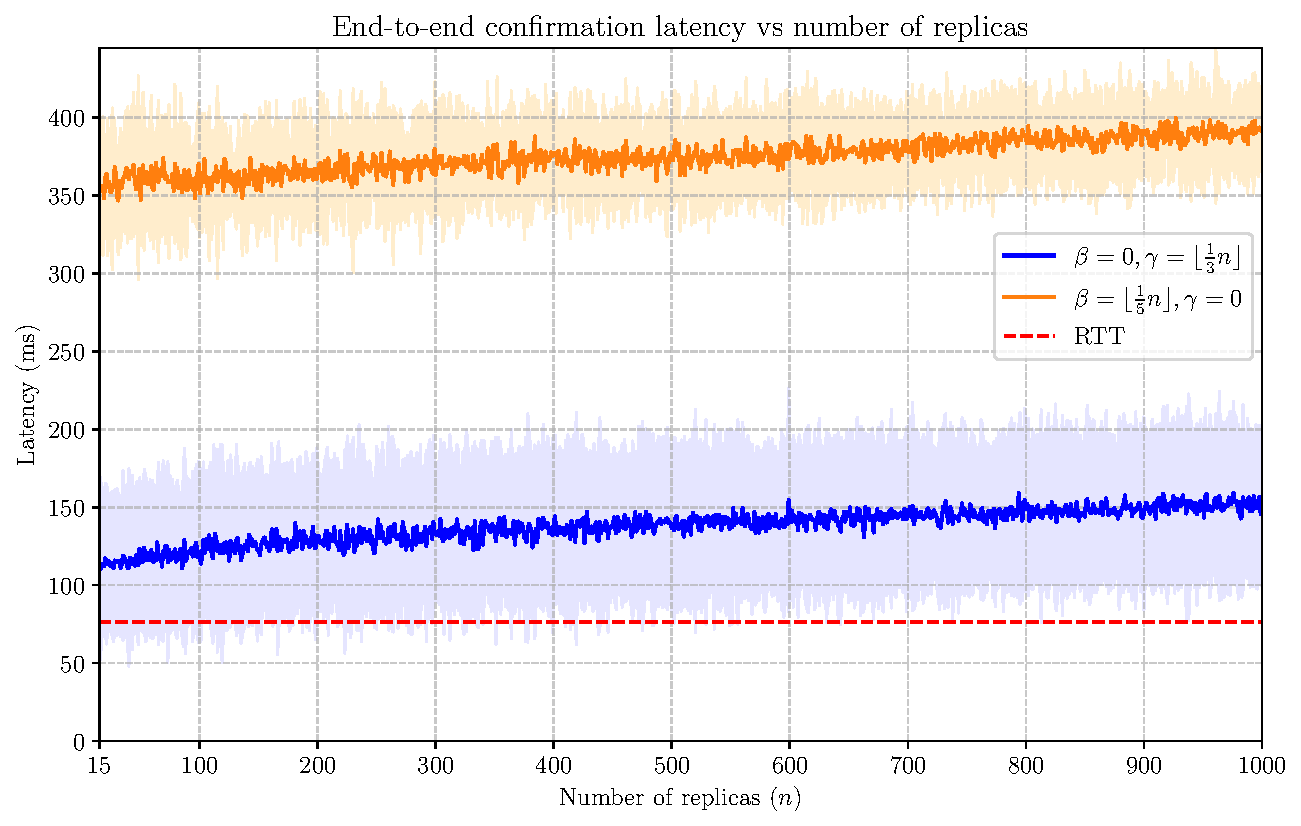
\includegraphics[width=0.9\textwidth]{figures/latency.pdf}
    \vspace{-5mm}
    \caption{End-to-end confirmation latency from a writing client to a reading client as a transaction traverses across $n = 15, \ldots, 1000$ replicas,
    for two reading clients:
    (1) a client that expects up to $\gamma = \lfloor\frac{1}{3}n\rfloor$ omission faults (blue line, below), and (2) a client that expects up to $\beta = \lfloor\frac{1}{5}n\rfloor$ Byzantine faults (orange line, above).
    The physical network round-trip time between the reading client and the writing client is also shown (dashed red line, 76ms).
    A 95\% confidence interval is shown (shaded).}
    \label{fig:latency}
\end{figure}
% \vspace{-5mm}

The implementation follows a client-server architecture where each replica maintains two TCP listening sockets:
one for the reading client connection and one for the writing client connection. Upon receiving a transaction
payload from a writer, the replica creates a tuple containing the payload, a sequence number, and the current local timestamp.
The replica then signs this tuple using a Schnorr signature\footnote{\url{https://crates.io/crates/secp256k1}} on secp256k1 curve, appends it to its local log, and forwards
the signed tuple to the reading client.
Replicas are deployed round-robin across seven
AWS regions: Frankfurt, London, N. Virginia, N. California, Canada, Mumbai, and Seoul. Each replica is deployed on a
t2.medium EC2 instance (2 vCPUs, 4GB RAM) and is initialized with user data that contains
the replica's unique secret signing key.

We implement two types of clients. The writing client establishes connections to all replicas, records
the timestamp (in its local view) right before sending the transaction and sends transaction
payloads to each replica. The reading client maintains connections to all replicas, validates incoming signed
transactions, and records the timestamp (in its local view) upon receiving a quorum of valid signatures for a particular transaction.
We deploy the reading
client in London and the writing client in N. Virginia, both initialized with the complete
list of replica information (IP addresses, public keys).

We conduct experiments with two different values for the quorum size $\alpha = 1 - \beta - \gamma$: (1) $\beta =0 $ and $\gamma = \lfloor \frac{1}{3} n \rfloor$, for a client that only expects omission faults,
and (2) $\beta = \lfloor\frac{1}{5}n\rfloor$ and $\gamma = 0$, for a client that expects Byzantine faults.
We repeat the experiments for
different numbers of replicas ($n = 15, \ldots, 1000$).
We repeat each experiment five times and report the mean latency and a 95\% confidence interval.

% To automate the deployment process, we dockerized the replica binary into a single image shared across all replicas.
% The entire deployment process is fully automated using the AWS SDK for Rust (aws-sdk-ec2 v1.17.0).
% The process handles instance creation, security group configuration, and user data initialization.
% creation, security group configuration, and user data initialization. This enables us to scale
% up to 1000 replicas with a single command.

As shown in Figure~\ref{fig:latency}, our experimental results demonstrate that the latency remains largely independent
of the number of replicas.
The reading client reports a transaction as confirmed as soon as the fastest
$\alpha$ replicas have responded, which gives rise to the happy artifact that the 1 - $\alpha$ slowest replicas
do not slow down confirmation.
This also explains why the omission-fault experiment exhibits lower latency than the Byzantine experiment.
Even with 1000 replicas the mean confirmation latency is 138ms for the omission-fault experiment and 375ms for the Byzantine experiment.
This approximates
the physical network round-trip time between the reading client and the writing client that stands at 76ms.

\section{Auctions on \podtm through the \bidsettm protocol}\label{sec:auctions}
In this section, we show how single-shot distributed auctions can be implemented on top of \podtm.
This is achieved through \bidsettm, a primitive for collecting a set of bids.
The idea is as follows. A pre-appointed \emph{sequencer} -- which can be any party, even a pod replica -- runs the auction, but the bids are collected from \podtm using a \bidsettm protocol. The past-perfection property of \podtm renders the sequencer unable to censor bids: when it creates an output, all timely and honestly-written bids \emph{must} be in it, otherwise the sequencer has provably misbehaved and can be held accountable.
% We first define \bidsettm and then construct it using an underlying \podtm.


\begin{definition}[\bidsettm protocol]\label{def:auction-framework}
    A \bidsettm \emph{protocol} has a \emph{starting time} parameter \tzero and exposes the following interfaces to \emph{bidder} and \emph{consumer} parties:
    \begin{itemize}
        \item function $\opSubmitBid{\bid}$: It is called by a bidder at round \tzero to submit a bid \bid.
        \item event $\opResult{\bag, \bidcert}$: It is an event generated by a consumer. It contains a \emph{bid-set} \bag, which is a set of bids, and auxiliary information \bidcert.
    \end{itemize}
\end{definition}


A \bidsettm protocol satisfies the following liveness and safety properties:
\begin{description}
    \item[(Liveness) Termination within \parAuctionTerm:]
    An honest consumer generates an event $\opResult{\bag, \bidcert}$ by round $\tzero + \parAuctionTerm$.

    \item [(Safety) Censorship resistance:]
    If an honest bidder calls \opSubmitBid{\bid}
    and an honest consumer generates an event $\opResult{\bag, $\cdot$}$,
    then $\bid \in \bag$.
    %  or a subset of the parties that run the \bidsettm protocol is accountable.
    % \hue{Bid inclusion: In a synchronous network, all honest bids are included}
    % Moreover, \emph{fair punishment} holds: an honest sequencer cannot be held accountable for censoring bids, even in asynchronous networks.
    % \oa{Notice that, even in asynchrony, an honest sequencer cannot be blamed, in the construction we present.}

    \item[(Safety) Weak consistency:]
    If two honest consumers generate \opResult{$\bag_1, \cdot$} and \opResult{$\bag_2, \cdot$} events, such that $\bag_1 \neq \emptyset$ and $\bag_2 \neq \emptyset$, then $\bag_1 = \bag_2$.
    % \hue{Single-result: If there are multiple conflicting auction results, the sequencer can be held accountable}
    % \oa{Only in synchrony.}

\end{description}

%As with previous protocols, we require that \bidsettm satisfies \emph{accountable safety}. This property means that, if a safety property is violated, then an \identify{} function returns a subset of the parties that run the \bidsettm protocol and are malicious, and that honest parties are never returned by \identify{}.

% \subsection{Construction}
%We present \bidsettm-core, a \bidsettm construction that uses a \podtm to register bids.

% We now present \bidsettm-core, a \bidsettm construction that uses \podtm-core to register bids.

\begin{protocol}[\bidsettm-core]\label{const:bidset}
	Construction \bidsettm-core is parameterized by an integer $\Delta$ (looking ahead, we will prove security in synchrony, \textit{i.e.}, assuming the network delay $\delta$ is smaller than $\Delta$) and assumes digital signatures and a \podtm with $\delta$-timeliness, $\parPerf=\delta$ and $\parConf=2\delta$. At time \tzero, bidders execute \Cref{alg:bid-set-bidder}, the sequencer \Cref{alg:bid-set-sequencer}, and the consumers \Cref{alg:bid-set-consumer}.
	% A bidder runs \opSubmitBid{} (\Cref{alg:bid-set-bidder}), the sequencer runs \opRunAuction{} (\Cref{alg:bid-set-sequencer}), and a consumer runs \opReadResult{} (\Cref{alg:bid-set-consumer}), in order to output the $\opResult{\bag, \bidcert}$ event.
	% A pre-appointed \emph{sequencer} is responsible to reading the \podtm and writing back to it when a specific condition is met. For example, when instantiating \bidsettm-core on top of \podtm-core, a replica can act as sequencer.
\end{protocol}

\vspace{-3mm}
\begin{algorithm}[]
    \caption{\bidsettm-core: Code for a bidder. It runs a client for a \podtm-core instance \podInst.}
    \label{alg:bid-set-bidder}
    \begin{algorithmic}[1]
        \Function{\opSubmitBid{\bid}}{}
            \State{\podInst.\opwrite{\bid}}
        \EndFunction
\end{algorithmic}
\end{algorithm}

\vspace{-3mm}
\begin{algorithm}[]
    \caption{\bidsettm-core: Code for the sequencer. It runs a client for a \podtm-core instance \podInst, and $\sk_a$ denotes the secret key of the sequencer.}
    \label{alg:bid-set-sequencer}
    \begin{algorithmic}[1]
        \Function{\opRunAuction{}}{}
            \Let{\left( (\txSet, \rperf), (\ppcert, \alltxcert) \right)}{\podInst.\opreadall{}}
            \While{$\rperf \leq \tzero + \Delta$}\label{line:bidset-wait-pp}
                \Let{\left( (\txSet, \rperf), (\ppcert, \alltxcert) \right)}{\podInst.\opreadall{}}
            \EndWhile{}
            \State{$\bag \gets \{\tx \mid (\tx, \cdot, \cdot , \cdot) \in \txSet\}  ;\; \bidcert \gets \ppcert$}\label{line:bidset-create-bag}
            \Let{\sigma}{\opSign{\sk_a, (\bag, \bidcert)}} \label{line:bidset-sequencer-sign}
            \Let{\tx}{\msgbidresult{(\bag, \bidcert, \sigma)}}\label{line:bidset-write-bag}
            \State{\podInst.\opwrite{\tx}} %Run by \tzero + 2 \Delta.
        \EndFunction
\end{algorithmic}
\end{algorithm}

\vspace{-3mm}
\begin{algorithm}[]
    \caption{\bidsettm-core: Code for a consumer. It runs a client for a \podtm-core instance \podInst.}
    \label{alg:bid-set-consumer}
    \begin{algorithmic}[1]
        \Function{\opReadResult{}}{}
            \Loop{}\label{line:bidset-wait-pp-consumer}
                \Let{((\txSet, \rperf), (\ppcert, \alltxcert))}{\podInst.\opreadall{}}
                    \If{$\exists (\tx, \cdot, \cdot, \rconf, \cdot) \in \txSet$ \textbf{:} $\tx = \msgbidresult{(\bag, \bidcert, \sigma)}$ \andl $\rconf \leq \tzero + 3 \Delta$} \label{line:bidset-find-confirmed-tx}
                    \State{\textbf{output event} \opResult{\bag, \bidcert}}
                \ElsIf{$\rperf > \tzero + 3 \Delta$}\label{line:bidset-read-result-pp}
                    \State{\textbf{output event} \opResult{$\emptyset$, \ppcert}}
                \EndIf
            \EndLoop\label{line:bidset-consumer-loop-end}
        \EndFunction
    \end{algorithmic}
    \end{algorithm}

% \vspace{-5mm}

A bidder (\Cref{alg:bid-set-bidder}) submits a bid by writing it on the \podtm  at round \tzero.
The sequencer (\Cref{alg:bid-set-sequencer}) waits until the \podtm returns a past-perfect round larger than $\tzero + \Delta$ (\cref{line:bidset-wait-pp}) and then constructs the bid-set \bag from the set of transactions in \txSet (\cref{line:bidset-create-bag}).
The sequencer concludes by signing \bag and \bidcert (which can be used as evidence, in case of a safety violation) and writing  \msgbidresult{(\bag, \bidcert, \sigma)} on \podInst.
The consumer (\Cref{alg:bid-set-consumer}) waits until one of the following two conditions is met.
First, a \emph{confirmed} transaction \msgbidresult{(\bag, \bidcert, \sigma)} appears in \txSet , for which $\rconf \leq \tzero + 3 \Delta$ (\cref{line:bidset-find-confirmed-tx}), in which case it outputs bid-set \bag as result.
Second, a round higher than $\tzero + 3 \Delta$ becomes past-perfect in \podtm (\cref{line:bidset-read-result-pp}) without a confirmed \msgbidresult{} transaction appearing, in which case it outputs $\bag=\emptyset$.

As an intuition on how \bidsettm-core achieves censorship resistance, we observe the following.
The \emph{$\delta$-timeliness property} of \podtm (\Cref{def:pod-timely}), given that $\delta \leq \Delta$, ensures that bids of honest parties will have a \confirmed round $\rconf \leq \tzero + \Delta$.
Now, the sequencer may only produce a valid bid-set when \podtm returns a past-perfect round larger than $\tzero + \Delta$ (\cref{line:bidset-wait-pp}), and the output \emph{must} contain a certificate \ppcert that proves this. However, if the certificate is valid, then the sequencer must have \emph{provably} seen the bids of honest parties in \txSet (we remind that the votes of replicas on \podtm-core are chained using sequence numbers), and thus \bag must contain all bids with $\rconf \leq \tzero + \Delta$. If any party presents a transaction certificate \txcert for some transaction $\tx^*$ with $\rconf^* \leq \tzero + \Delta$, but $\tx^* \not\in \bag$, then the sequencer can be held accountable.
% We show the detailed proof in \Cref{lem:bidset-censorship} and \Cref{lem:bidset-accountability}.

% Regarding liveness, \cref{line:bidset-wait-pp} of \Cref{alg:bid-set-sequencer} becomes true in the view of sequencer by round $\tzero + \Delta + \delta$ (from the \emph{past-perfection within $\parPerf=\delta$} property of \podtm-core),
% hence \Cref{alg:bid-set-sequencer} for an honest sequencer terminates by that round.
% Observe also that the transaction \msgbidresult{(\bag, \bidcert, \sigma)} becomes confirmed in the view of all honest clients by round $\tzero + \Delta + 3\delta$ (from the \emph{confirmation within $\parConf=2\delta$} property), and it will have a confirmed round $\rconf \leq \tzero + \Delta + 2\delta$ (from the \emph{$\delta$-timeliness} property).
% Hence, if the network is synchronous and the sequencer honest, the condition in \cref{line:bidset-find-confirmed-tx} of \Cref{alg:bid-set-consumer} becomes true at round at most $\tzero + \Delta + 3\delta$,
% Even if the sequencer is malicious, from the \emph{past-perfection within $\parPerf=\delta$} property of \podtm, the condition in \cref{line:bidset-read-result-pp} will become true at latest at round $\tzero + 3 \Delta + \delta$, hence \bidsettm-core achieves \emph{termination within $\parAuctionTerm=3\Delta + \delta$}.

% hence it outputs \bag as the bid-set, hence \bidsettm-core satisfies the \emph{consistency} property.




\begin{theorem}[Bidset security]\label{thm:bidset-construction-secure}
Assuming a synchronous network where $\delta \leq \Delta$,
protocol \bidsettm-core (Construction~\ref{const:bidset}) instantiated with a digital signature and a  secure \podtm protocol that satisfies the \emph{past-perfection within $\parPerf = \delta$}, \emph{confirmation within $\parConf=2\delta$} and \emph{$\delta$-timeliness} properties, is a secure \bidsettm protocol satisfying \emph{termination within $\parAuctionTerm = 3\Delta + \delta$}.
It satisfies accountable safety with an \identifySequencer{} function that identifies a malicious sequencer.
\end{theorem}
\vspace{-3mm}
\begin{proof} The proof and \identifySequencer{} are shown in Appendix~\ref{app:bidsetsec}.
\end{proof}

\begin{remark}
    Observe that \bidsettm-core terminates within $\parAuctionTerm = 3\Delta + \delta$ in the worst case, but, if the sequencer is honest, then it terminates within $\parAuctionTerm = \Delta + 3\delta$.
    Moreover, \bidsettm-core is not responsive because \Cref{alg:bid-set-sequencer} waits for a fixed $\Delta$ interval.
    This step can be optimized if the set of bidders is known (e.g., requiring them to pre-register), which allows for the protocol to be made optimistically responsive (\textit{i.e.}, $\parAuctionTerm = 4\delta$) when all parties are honest.
\end{remark}

\begin{remark}[Implicit sub-session identifiers]
	We assume that each instance of the \bidsettm-core protocol is identified by a unique sub-session identifier (ssid). All messages written to the underlying \podtm are concatenated with the ssid.
\end{remark}

\dotparagraph{\textbf{Auctions using \bidsettm}} Building on a \bidsettm protocol, it is trivial to construct single-shot first-price and second-price open auctions as follows: 1. Bidders place their open bids $\bid$ by calling \opSubmitBid{\bid}; 2. Consumers determine the winner by calling \opReadResult{} to obtain $\bag$ and outputting either the first or second highest bid. We conjecture that single-shot sealed bid auction protocols such as those of~~\cite{trustee,seal,ACNS:DavGenPou22,CCS:TAFWBM23,chitra_et_al:LIPIcs.AFT.2024.19,cryptoeprint:2024/1011} can also be instantiated on top of a \bidsettm protocol. Intuitively, this holds because such protocols first agree on a set of sealed bids and then execute extra steps to determine the winner. However, a formal analysis of sealed-bid auction protocols based on \bidsettm is left as future work.

\section{Conclusion}
%"novel consensus layer that finalizes transactions with the optimal one-round-trip latency" sounds a bit fluffy, let's make this more precise for the DISC submission, or just remove this Discussion section.
In this work we present \podtm, a novel consensus layer that finalizes transactions with the optimal one-round-trip latency by eliminating communication among replicas. Instead, clients read the system state by performing lightweight computation on logs retrieved from the replicas. As no validator has a particular role in \podtm (as compared to leaders, block proposers, miners, etc. in similar protocols), \podtm achieves censorship resistance by default, without any extra mechanisms or additional cost. Furthermore, validator misbehavior, such as voting in incompatible ways or censoring confirmed transactions, is accountable.

As an application, we present an efficient and censorship-resistant mechanism for single-shot first-price and second-price open auctions, which leverages \podtm as a bulletin board.
We show how the accountability, offered by \podtm, is also inherited by applications built on it -- the auctioneer cannot censor confirmed bids without being detected.
In the full version~\cite{DBLP:journals/corr/abs-2501-14931} of this paper we discuss further applications, including payments in the style of Fastpay~\cite{DBLP:conf/aft/BaudetDS20}.

We conjecture that single-shot sealed bid auction protocols, such as those of~\cite{trustee,seal,ACNS:DavGenPou22,CCS:TAFWBM23,chitra_et_al:LIPIcs.AFT.2024.19,cryptoeprint:2024/1011}, can also be instantiated on top of a \bidsettm protocol. Intuitively, this holds because such protocols first agree on a set of sealed bids and then determine the winner. A formal analysis of sealed-bid auction protocols based on \bidsettm is left as future work.
The architecture of \podtm also motivates the design of light clients, which would not have to connect to all replicas or to download all transactions. This is achieved through cryptographic primitives such as Merkle mountain ranges and segment trees. We leave the formal description as future work.

Finally, we remark that \podtm differs from standard notions of consensus because it does not offer an agreement property, neither to validators nor to clients. A client reading the \podtm obtains a past-perfect round \rperf, and it is guaranteed to have received all transactions that obtained a confirmed round \rconf such that $\rconf \leq \rperf$, or that may obtain such an $\rconf$ in the future, even though the transaction presently appears to the client as unconfirmed. However, the client cannot tell which unconfirmed transactions will become confirmed. Moreover, a transaction might appear confirmed to one client and unconfirmed to another (in this case, this is a transaction written by a malicious client).

% \vfill
% \pagebreak
% \pdfbookmark[section]{References}{references}
\bibliographystyle{plainurl}
\bibliography{abbrev3,crypto,biblio}

\appendix
% \section{Definition of \podtm monotonicity}\label{app:monotonicity}
% We define \emph{\podtm monotonicity} as an intermediate notion that stands between a simple secure \podtm and a $\theta$-timely \podtm. \oa{I am not sure this is true, or at least intuitive. I would remove this sentence.}

The property of \podtm monotonicity requires that, as time advances, $\rmin$ does not decrease, $\rmax$ does not increase and confirmed transactions remain confirmed.

\begin{definition}[\podtm monotonicity]
	A \podtm protocol satisfies \emph{pod monotonicity}, and is called a \emph{monotone \podtm}, if it is a secure \podtm, as per Definition~\ref{def:podsec}, and the following properties hold for any rounds $\round_1,\round_2 > \round_1$ and for any honest client~\client:
	\begin{description}
		\item [Past-perfection monotonicity:] It holds that $\podView{\client}{\round_2}.\rperf \geq \podView{\client}{\round_1}.\rperf$.
		\item [Transaction monotonicity:] If  transaction $\tx$ appears in $\podView{\client}{\round_1}.\txSet$, then $\tx$ appears in $\podView{\client}{\round_2}.\txSet$.
		\item [Confirmation-bounds monotonicity:] For every $\tx$ that appears in $\podView{\client}{\round_1}.\txSet$ with $\rmin,\rmax,\rconf$ and appears in  $\podView{\client}{\round_2}.\txSet$ with $\rmin',\rmax',\rconf'$,  it holds that $\rmin'\geq \rmin$, $\rmax' \leq \rmax$.
		% $\rconf' \geq \rconf$.

	\end{description}
\end{definition}

We now observe that a monotone \podtm protocol can be obtained from any secure \podtm protocol with stateful clients, and that monotonicity implies certain specific properties that may be useful for applications. In particular, our \podtm-core protocol naturally satisfies this property.

\begin{remark}
	Every secure \podtm can be transformed into a monotone \podtm if parties are stateful. Let $\round_1$ be the last round when an honest client $\client$ read the \podtm obtaining view $\podView{\client}{\round_1}$, which is stored as state until $\client$ reads the \podtm again. At any round $\round_2>\round_1$, if $\client$ reads the \podtm and obtains $\podView{\client}{\round_2}$, $\client$ can define a view $\overline{\podView{\client}{\round_2}}$ satisfying the properties of \podtm monotonicity:

	\begin{enumerate}
		\item If $\tx$ appears in $\podView{\client}{\round_1}$ with $\tx.\rmin,\tx.\rmax,\tx.\rconf,\tx.\txcert$, then $\tx$ appears in $\overline{\podView{\client}{\round_2}}$ with $\tx.\overline{\rmin}=\rmin,\tx.\overline{\rmax}=\rmax,\tx.\overline{\rconf}=\rconf,\tx.\overline{\txcert}=\txcert$.
		\item If $\tx$ appears in $\podView{\client}{\round_2}$ with $\tx.\rmin',\tx.\rmax',\tx.\rconf',\tx.\txcert'$ and does not appear in $\podView{\client}{\round_1}$, then $\tx$ appears in $\overline{\podView{\client}{\round_2}}$ with $\tx.\overline{\rmin}=\rmin',\tx.\overline{\rmax}=\rmax',\tx.\overline{\rconf}=\rconf',\tx.\overline{\txcert}=\txcert'$.
		\item For every $\tx$ that appears in $\podView{\client}{\round_1}.\txSet$ and in  $\podView{\client}{\round_2}.\txSet$ such that $\rmin'\geq \rmin$, $\rmax' \leq \rmax$, $\rconf' \geq \rconf$, update $\tx.\overline{\rmin}=\rmin',\tx.\overline{\rmax}=\rmax',\tx.\overline{\rconf}=\rconf',\tx.\overline{\txcert}=\txcert'$.
		\item If  $\podView{\client}{\round_2}.\rperf > \podView{\client}{\round_1}.\rperf$, then $\overline{\podView{\client}{\round_2}}.\rperf=\podView{\client}{\round_2}.\rperf $. Otherwise, $\overline{\podView{\client}{\round_2}}.\rperf=\podView{\client}{\round_1}.\rperf $.

	\end{enumerate}
\end{remark}

In the remarks below, we observe that \podtm monotonicity implies a number of useful properties about the monotonicity of past perfection and the values $\rmin,\rmax,\rconf$ associated to a transaction in the \podtm.

\begin{remark}[Confirmation monotonicity]\label{rem:confstick}
	Properties 2 and 3 of \podtm monotonicity imply that  for any honest client $\client$ and rounds $\round_1, \round_2 > \round_1$,
	if $\tx \in \podView{\client}{\round_1}$ and $\tx.\rconf \neq \bot$, then $\tx \in \podView{\client}{\round_2}$ and $\tx.\rconf \neq \bot$.
\end{remark}

\begin{remark}
	Observe that the \emph{confirmation monotonicity} property in Remark~\ref{rem:confstick} is a specific version of a more general \emph{common subset} property, which would demand the condition for any two honest clients $\client_1, \client_2$.
\end{remark}
\section{Validation function for \podtm-core}\label{sec:pod-core-valid}
In this section we present the function \opValid{}, which allows a \podtm client, which is not necessarily communicating with the \podtm replicas, to verify that a given pod data structure \Pod satisfies the security properties of \podtm (\Cref{def:podsec}).

\begin{algorithm}[]
    \caption{Function \opValid{\Pod, \cert} for \podtm-core. Code for a \emph{verifier}, which can be a pod client not communicating with the pod replicas.}
    \label{alg:pod-core-valid}
    \begin{algorithmic}[1]
        \State{\textbf{State:} Same as in \Cref{alg:client-1}, includes $\{\rep_1, \ldots, \rep_n\}$, \tsps, \mrt.}
        \Statex
        \vspace{-1mm}
        \Function{\opValid{\Pod, \cert}}{}
            \Let{(\ppcert, \alltxcert) }{\cert} \label{line:valid-extract-cert} \Comment{$\ppcert: \rep \rightarrow \vote, \; \alltxcert: \tx \rightarrow \txcert, \; \txcert: \rep \rightarrow \vote$}
            \State{\opInitClient{}} \Comment{shown in \Cref{alg:client-1}}
            \Let{\allVotes}{\bigcup_{\tx \in \alltxcert} \left(\alltxcert[\tx].\opValues{}\right)}
            \For{$(\tx, \tsp, \sn, \sig, \rep_j) \in \allVotes$ \textbf{in increasing order of} $\sn$}
                \State{\textbf{require} \opProcessVote{$\tx, \tsp, \sn, \sig, \rep_j$}} \Comment{shown in \Cref{alg:client-1}, updates \tsps, \mrt}
            \EndFor
            \State{\textbf{require} $\Pod.\txSet = \opComputeTxSet{\tsps, \mrt}$} \label{line:valid-check-begin} \Comment{shown in \Cref{alg:client-statistics}}
            \State{\textbf{require} $\Pod.\rperf = \opMinPossibleTsForNewTx{\mrt}$} \label{line:valid-check-end} \Comment{shown in \Cref{alg:client-statistics}}
            \For{$(\tx, \tsp, \sn, \sig, \rep_j) \in \ppcert.\opValues{}$} \label{line:valid-check-ppcert-begin}
                \State{\textbf{require} $(\tx, \tsp, \sn, \sig, \rep_j) \in \allVotes$}
                \State{\textbf{require} $\sn = \op{max}_{\sn'}((\cdot, \cdot, \sn', \cdot, \rep_j) \in \allVotes)$}
            \EndFor\label{line:valid-check-ppcert-end}
        \EndFunction
    \end{algorithmic}
    \end{algorithm}

The function \opValid{} for \podtm-core is shown in \Cref{alg:pod-core-valid}.
The idea is to have the verifier repeat the logic of an honest client.
The verifier is initialized in the same way as in \Cref{alg:client-1} -- importantly, it knows the identifiers and public keys of \podtm replicas.
Function \opValid{} takes as input a \podtm data structure \Pod and auxiliary data \cert,
which contains two parts, a \emph{past-perfection certificate} \ppcert and a collection of \emph{transaction certificates} $\alltxcert$, one for each transaction in \Pod.\txSet.
Both contain vote messages, as constructed by a \podtm client in lines \ref{line:upd-ppcert} and \ref{line:client-store-vote-txcert} of \Cref{alg:client-1}.
The verifier processes each vote in order of increasing sequence number \sn using function \opProcessVote{}. If any vote is invalid, \opValid{} returns $\false$.
Observe that if the votes are valid the verifier will have updated its local \tsps and \mrt variables with the same values as the \podtm client that constructed \Pod.
Finally, the verifier computes the transaction set \txSet and the past-perfect round \rperf (using its local \tsps and \mrt variables) and requires that the values match the ones in \Pod (lines~\ref{line:valid-check-begin}--\ref{line:valid-check-end}).

Finally, the verifier also verifies the past-perfection certificate. Given that the previous checks have passed, we require that each vote in \ppcert is contained in one of the transaction certificates in \alltxcert and has the maximum sequence number received from the client that sent the vote (lines~\ref{line:valid-check-ppcert-begin}--\ref{line:valid-check-ppcert-end}).
As we have remarked earlier, \ppcert can be derived from \alltxcert by taking the union of certificates $\alltxcert$ for all transactions and keeping the most recent vote for each replica, in which case the checks on lines~\ref{line:valid-check-ppcert-begin}--\ref{line:valid-check-ppcert-end} can be omitted. We maintain the past-perfection certificate for readability and simplicity in the proofs.
\section{Security of Protocol \podtm-core under a Continuum of Byzantine and Omission faults}\label{app:pod-security}
In order to prove Theorem~\ref{thm:pod-security} and establish the security of Protocol \podtm-core shown Construction~\ref{const:pod-core}, we first prove some useful intermediate results. We remind that $n = \alpha + \beta + \gamma$, where $n$ denotes the total number of replicas, $\beta$ denotes the number of Byzantine replicas, \gamma denotes the number of omission-faulty replicas in an execution, and \alpha denotes the number of replicas required to confirm a transaction.

\begin{lemma}[The values for minimum, maximum and \confirmed rounds]\label{lem:assign-min-max}
	Regarding \Cref{alg:client-statistics}, we have the following.
	Consider the list of all timestamps received by a client for a particular transaction, replacing a missing vote from $\rep_j$ with a special value ($\mrt[\rep_j]$ for computing \rmin, $\infty$ for computing \rmax), to get $n$ values in total, sorted in increasing order.
	Assume \mrt is also sorted in increasing order of timestamps.
	\begin{enumerate}
		\item \rmin is the timestamp at index $\lfloor \alpha / 2 \rfloor - \beta$ of this list.
		\item \rmax is the timestamp at index $n - \alpha + \lfloor \alpha / 2 \rfloor + \beta$ of this list.
		\item \rperf is the timestamp at index $\lfloor \alpha / 2 \rfloor - \beta$ of \mrt.
	\end{enumerate}
\end{lemma}
\begin{proof}
	Functions \opMinPossibleTs{} and \opMinPossibleTsForNewTx{} prepend \beta times the $0$ value in the beginning of the list and return the median of the first \alpha values, hence they return the timestamp at index $\lfloor \alpha / 2 \rfloor - \beta$.
	Function \opMaxPossibleTs{} appends \beta times the $\infty$ value at the end of the list and returns the median of the last \alpha values of that list, that is, it ignores the first $n - \alpha  + \beta$ values and returns the timestamp at index $n - \alpha  + \beta + \lfloor \alpha / 2 \rfloor$.
\end{proof}

\begin{lemma}[\rperf bounded by honest timestamp]\label{lem:rperf-value-of-honest}
	Assuming $n \geq 5 \beta + 3 \gamma + 1$ (equiv., $\alpha \geq 4\beta + 2 \gamma + 1$),
	% if $\opValid{\Pod, \cert} = \true$ for some pod data structure \Pod and auxiliary data $\cert = (\ppcert, \{\txcerti{i}\}_{i=0}^m)$,
	for a valid pod \Pod with auxiliary data $\cert = (\ppcert, \alltxcert)$,
	there exists some honest replica $\rep_j$, such that the most-recent timestamp \mrt from $\rep_j$ included in $\ppcert$ satisfies $\mrt \leq \Pod.\rperf$.
\end{lemma}
\begin{proof}
	Since $\opValid{\Pod, \cert} = \true$, the past-perfect round $\Pod.\rperf$ is the value returned by \opMinPossibleTsForNewTx{} of \Cref{alg:client-statistics}.
	From \Cref{lem:assign-min-max} we have that \rperf is the timestamp at index $\lfloor \alpha / 2 \rfloor - \beta$ of sorted \mrt.
	The condition $\alpha \geq 4\beta + 2 \gamma + 1$ implies that $\beta + \gamma \leq \lfloor \alpha / 2 \rfloor - \beta$,
	hence the number of not honest replicas ($\beta + \gamma$) cannot fill all positions between $0$ and $\lfloor \alpha / 2 \rfloor - \beta$,
	hence at least one of the indexes between $0$ and $\lfloor \alpha / 2 \rfloor - \beta$ (inclusive) will
	contain the timestamp created and sent by an honest replica.
\end{proof}
% \begin{lemma}\label{lemma:number-votes-in-cert}
	%     For a $\Pod.\rperf$, we have that
	%     \begin{enumerate}
		%         \item
		%         \item If some transaction $\tx \in \Pod$ is assigned $\rmax \neq \infty$ as the maximum round,
		%         then \Pod contains votes on \tx from at least $n - \lfloor \alpha / 2 \rfloor - 1$ honest replicas with a timestamp $\tsp \leq \rmax$.
		%         \item There are at most $\lceil \alpha / 2 \rceil - \beta - 1$ replicas for which the most-recent timestamp satisfies  $\mrt < \rperf$,
		%         and at least $n - \lceil \alpha / 2 \rceil + \beta + 1$ replicas from which a vote with timestamp $\tsp \geq \Pod.\rperf$ is included in \Pod.
		%     \end{enumerate}
	% \end{lemma}
% \begin{proof}
	%     \begin{enumerate}
		%         \item
		%         \item From \Cref{lem:assign-min-max}, the list with all returned timestamps contains $n - \alpha  + \beta + \lceil \alpha / 2 \rceil - 1$ elements smaller or equal to \rmax,
		%         and, since $\rmax \neq \infty$, at least $n - \alpha  + \lceil \alpha / 2 \rceil - 1 = n - \lfloor \alpha / 2 \rfloor - 1$
		%         of them are timestamps returned by honest parties.
		%         \oa{TODO: The equivalent of this is $2f$. We would ideally like it to be $2f+1$. Check again.}
		%         \item It follows from \Cref{lem:assign-min-max}, as \rperf is the ($\lceil \alpha / 2 \rceil - \beta$)-th smallest value in \mrt.
		%     \end{enumerate}
	% \end{proof}

\noindent

We now recall Theorem~\ref{thm:pod-security}, which we prove through a series of lemmas.

\begin{customthm}{\ref{thm:pod-security}}[\podtm-core security]
	Assume that the network is partially synchronous with actual network delay $\delta$, that \beta is the number of Byzantine replicas, \gamma the number of omission-faulty replicas, $\alpha = n - \beta - \gamma$ the confirmation threshold, and $n \geq 5 \beta + 3 \gamma + 1$ the total number of replicas. Protocol \podtm-core (\Cref{const:pod-core}), instantiated with a EUF-CMA secure signature scheme, the \opValid{} function shown in \Cref{alg:pod-core-valid}, and the \identify{} function described in \Cref{alg:identify}, is a responsive secure \podtm (\Cref{def:podsec}) with Confirmation within $\parConf = 2 \delta$, Past-perfection within $\parPerf = \delta$ and  \beta-accountable safety (\Cref{def:accountable-safety}), \ewnp.
\end{customthm}
\begin{proof}
	The proof follows from Lemmas~\ref{lem:pod-confirmation}--\ref{lem:pod-accountable-safety}, presented and proven in the remainder of this section.
\end{proof}

\begin{lemma}[Confirmation within $\parConf$]\label{lem:pod-confirmation}
	For the conditions stated in \Cref{thm:pod-security}, \Cref{const:pod-core} satisfies the \emph{confirmation within $\parConf$} property (\Cref{def:podsec}) for $\parConf = 2 \delta$.
\end{lemma}
\begin{proof}
	Assume an honest client \client calls \opwrite{\tx} at round \round.
	It sends a message \msgwrite{\tx} to all replicas at round \round (line~\ref{line:send-write-tx}).
	An honest replica receives this by round $\round + \delta$ and sends a \msgrecord{} message back to all connected clients (line~\ref{line:send-vote}).
	An honest client $\client'$ receives the vote by round $\round + 2\delta$.
	As are at least \alpha honest (not Byzantine and not omission-faulty) replicas, $\client'$ receives at least \alpha such votes, hence the condition in line~\ref{line:confirm-tx-begin} is satisfied and $\client'$ observes \tx as \confirmed.
\end{proof}

\begin{lemma}[Past-perfection within $\parPerf$]\label{lem:past-perfection-liveness}
	For the conditions stated in \Cref{thm:pod-security}, \Cref{const:pod-core} satisfies the \emph{past-perfection within $\parPerf$} property (\Cref{def:podsec}) for $\parPerf = \delta$.
\end{lemma}
\begin{proof}
	Assume an honest client \client at round \round has view $\podView{c}{\round}$.
	From \Cref{lem:rperf-value-of-honest}, there exists some honest replica $\rep_j$, such that the most-recent timestamp $\mrt[\rep_j]$ that $\rep_j$ has sent to \client satisfies $\podView{c}{\round}.\rperf \geq \mrt[\rep_j]$.
	The honest replica $\rep_j$ sends at least one heartbeat or vote message per round (line~\ref{line:rep-send-vote-heartbeat}), which arrives within $\delta$ rounds, and an honest client updates $\mrt[\rep_j]$ when it receives the heartbeat or vote message.
	Hence, \client will have $\mrt[\rep_j] \geq \round - \delta$.
	All together, $\podView{c}{\round}.\rperf \geq \round - \delta$.
\end{proof}

% \begin{lemma}[Confirmation stickiness]
	%     \Cref{const:pod-core} satisfies the \emph{confirmation stickiness} property.
	% \end{lemma}
% \begin{proof}
	%     It follows from the fact that clients in \Cref{const:pod-core} are \emph{stateful} and operation \opread{} (lines~\ref{line:read-begin}--\ref{line:read-end}) operates on local state.
	%     If \opread{} returns a set of transaction \transactions which contains a \confirmed transaction \tx, then \transactions will contain this \tx as confirmed in any subsequent call to \opread{}.
	%     % This implies that \tx got assigned an $\rconf \neq \bot$ in line~\ref{line:assign-median}, which implies the condition in line~\ref{line:confirm-tx-begin} was at some point true. As the structure \tsps is persisted across calls to \opread{}, any subsequent \opread{} will return \tx as \confirmed.
	% \end{proof}
\begin{lemma}[Past-perfection safety]\label{lem:pod-pp-safety}
	For the conditions stated in \Cref{thm:pod-security}, \Cref{const:pod-core} satisfies the \emph{past-perfection} safety property (\Cref{def:podsec}), except with negligible probability.
\end{lemma}
\begin{proof}
	Assume the adversary outputs valid $(\Pod_1, \cert_1)$ and $(\Pod_2, \cert_2)$ that violate the property,
	i.e., there exists a transaction $\tx$ such that $(\tx, \rmin^1, \rmax^1, \rconf^1) \not\in \Pod_1.\txSet$ and $(\tx, \rmin^2, \rmax^2, \rconf^2) \in \Pod_2.\txSet$ and $\rconf^2 \neq \bot$ and $\rconf^2 < \Pod_1.\rperf$.
	Let $\cert_1 = (\ppcert^1, \alltxcert^1)$ and $\cert_2 = (\ppcert^2, \alltxcert^2)$.

	% Assume an honest client $\client$ at round $\round > 0$ reads the \podtm and obtains $(\txSet, \rperf, \ppcert)$.
	% such that $\tx \not \in \txSet$, for some $\tx \in \zo^*$.
	% Let $\allreps_1$ be the set of replicas $\rep_i$ for which $\client$ stores at round $\round$ an $\mrt_i \geq \rperf$.
	Let $\allreps_1$ be the set of replicas $\rep_i$ for which $\ppcert^1$ contains a vote with timestamp $\mrt_i \geq \Pod_1.\rperf$.
	From \Cref{lem:assign-min-max} (\rperf is computed as the timestamp at index $\lfloor \alpha / 2 \rfloor - \beta$ of sorted \mrt), and since $\Pod_1$ is valid, there exist at least $n - \lfloor a/2 \rfloor + \beta$ such replicas, hence $|\allreps_1| \geq n - \lfloor a/2 \rfloor + \beta$.
	% Observe that no replica in $\allreps_1$ has sent to $\client$ a vote on \tx (because $\tx \not \in \txSet$),
	For each $\rep_i \in \allreps_1$, the transaction certificates $\alltxcert^1$ contain the whole log of $\rep_i$ with timestamps up to $\mrt_i$ (\cref{line:client-check-sn} of \Cref{alg:client-1} does not allow gaps in the sequence number of the received votes).
	That is, for each $\rep_i \in \allreps_1$ the certificates $\alltxcert^1$ contains votes
	%
	\begin{equation}\label{eq:proof-pp-set1}
		(\tx_{i,1}, \tsp_{i,1}, 1, \sigma_{i,1}, \rep_i), (\tx_{i,2}, \tsp_{i,2}, 2, \sigma_{i,2}, \rep_i), \ldots, (\tx_{i,k_i}, \tsp_{i, k_i}, k_i, \sigma_{i, k_i}, \rep_i),
	\end{equation}
	%
	where $k_i$ is the smallest sequence number for which $\tsp_{i, k_i} \geq \Pod_1.\rperf$, and $\tx_{i,j}$ are transactions.

	% Assume another client $\client'$ at some round $\round' > 0$ outputs a \podtm $(\txSet', \cdot, \cdot)$,
	% such that $(\tx, \cdot, \cdot, \rconf, \txcert) \in \txSet'$ and $\rconf < \rperf$ (where \rperf is the past-perfect round observed by $\client$).
	Since \tx is confirmed in $\Pod_2$ and $\rconf^2 < \Pod_1.\rperf$, the transaction certificate $\alltxcert^2[\tx]$ must contain votes on \tx with timestamp $\tsp_i$, such that $\tsp_i < \Pod_1.\rperf$, from at least $\lfloor \alpha/2 \rfloor + 1$ replicas.
	Let $\allreps_2$ be the set of these replicas, with $|\allreps_2| \geq \lfloor \alpha/2 \rfloor + 1$.
	For each $\rep_i \in \allreps_2$, certificate $\alltxcert^2[\tx]$ contains a vote
	%
	\begin{equation}\label{eq:proof-pp-vote2}
		(\tx, \tsp_i, \sn_i, \sigma_i, \rep_i),
	\end{equation}
	%
	such that $\tsp_i < \Pod_1.\rperf$.
	We will show that, if at most \beta replicas are Byzantine, this leads to a contradiction.
	% Observe that an honest replica cannot be in both $\allreps_1$ and $\allreps_2$, because that would imply that it omitted sending a vote to \client.
	Observe from the cardinality of $\allreps_1$ and $\allreps_2$ that at least $\beta + 1$ replicas must be in both sets, hence at least one honest replica must be in both sets (except if the adversary forges a signature under the public key of an honest replica, which happens with negligible probability).
	For that replica, the vote in (\ref{eq:proof-pp-vote2}) must be one of the votes in (\ref{eq:proof-pp-set1}) since $\tsp_i < \Pod_1.\rperf$ and $\tsp_{i, m_i} \geq \Pod_1.\rperf$.
	Hence, one of the $\tx_{i,j}$ in (\ref{eq:proof-pp-set1}) is \tx, and $\tx$ must appear in $\Pod_1.\txSet$, a contradiction.
\end{proof}

% \begin{lemma}[Past-perfection monotonicity]
	%     \Cref{const:pod-core} satisfies the \emph{past-perfection monotonicity} property.
	% \end{lemma}
% \begin{proof}
	%     It follows from the fact that clients in \Cref{const:pod-core} use a stateful construction,
	%     and the fact that the most-recent timestamps can only increase.
	% \end{proof}

\begin{lemma}[Confirmation bounds]\label{lem:bounds-safety}
	For the conditions stated in \Cref{thm:pod-security}, \Cref{const:pod-core} satisfies the \emph{confirmation bounds} safety property (\Cref{def:podsec}), except with negligible probability.
\end{lemma}
\begin{proof}
	Assume the adversary outputs $(\Pod_1, \cert_1)$ and $(\Pod_2, \cert_2)$, such that $\opValid{\Pod_1, \cert_1} \land \opValid{\Pod_2, \cert_2}$ and there exists a transaction $\tx$ such that $(\tx, \rmin^1, \rmax^1, \rconf^1) \in \Pod_1.\txSet$ and $(\tx, \rmin^2, \rmax^2, \rconf^2) \in \Pod_2.\txSet$.
	Let $\cert_1 = (\ppcert^1, \alltxcert^1)$ and $\cert_2 = (\ppcert^2, \alltxcert^2)$, and $\txcert^1 = \alltxcert^1[\tx]$ and $\txcert^2 = \alltxcert^2[\tx]$.

	First assume $\rmin^1 > \rconf^2$.
	% Assume client $\client_1$ computes \rmin and client $\client_2$ computes $\rconf < \rmin$ for \tx.
	From \Cref{lem:assign-min-max}, $\txcert^1$ can include at most $\lfloor \alpha / 2 \rfloor - \beta$ votes with a timestamp for \tx smaller than $\rmin^1$.
	Allowing up to \beta replicas to equivocate, the adversary can obtain at most $\lfloor \alpha / 2 \rfloor$ votes on \tx with a timestamp smaller than $\rmin^1$, except if it forges a digital signature from an honest replica, which happens with negligible probability.
	In order to compute $\rconf^2 < \rmin^1$ for \tx, the adversary must include in $\txcert^2$ timestamps smaller than $\rmin^1$ from at least $\lfloor \alpha / 2 \rfloor + 1$ replicas.

	Now assume $\rmax^1 < \rconf^2$.
	% For \rmax, assume $\client_1$ computes \rmax and $\client_2$ computes $\rconf > \rmax$.
	Using \Cref{lem:assign-min-max}, $\txcert^1$ can include at most $\alpha - \lfloor \alpha / 2 \rfloor - \beta - 1$ votes with a timestamp larger than \rmax,
	hence the number of honest replicas, from which a vote with timestamp larger than \rmax can be included in $\txcert^2$ is at most $\alpha - \lfloor \alpha / 2 \rfloor - 1$ (since \beta are malicious).
	If \alpha is odd, this upper bound becomes $\alpha - \lfloor \alpha / 2 \rfloor -1 = \lfloor \alpha / 2 \rfloor $, while at least
	$\lfloor \alpha / 2 \rfloor + 1$ votes larger that \rmax are required to compute a median larger than \rmax,
	and if \alpha is even, then $\alpha - \lfloor \alpha / 2 \rfloor - 1 = \lfloor \alpha / 2 \rfloor - 1$, while at least
	$\lfloor \alpha / 2 \rfloor$ votes larger that \rmax are required to compute a median larger than \rmax.
	(we remind that \cref{alg:client-statistics} returns as median the value at position $\lfloor \alpha /  2 \rfloor$).
	In either case, we get a contradiction, except for the negligible probability that the adversary forges a digital signature from an honest replica.
\end{proof}

\begin{algorithm}[]
    \caption{The \identify{} function for Protocol \podtm-core (\Cref{const:pod-core}).}
    \label{alg:identify}
    \begin{algorithmic}[1]
        \Function{\identify{\tran}}{}
            \Let{\cheaters}{\emptyset}
            % \For{$ \msgrecord{(\tx_1, \tsp_1, \sn_1, \sig_1, \rep_1)},\; \msgrecord{(\tx_2, \tsp_2, \sn_2, \sig_2, \rep_2)} \in \tran$}
            \For{$ \msgrecord{(\tx_1, \tsp_1, \sn_1, \sig_1, \rep_1)} \in \tran$}
                \If{\textbf{not} \opVerify{$\pk_1, (\tx_1, \tsp_1, \sn_1), \sig_1$}}
                    \State{\textbf{continue}}
                \EndIf
                \For{$ \msgrecord{(\tx_2, \tsp_2, \sn_2, \sig_2, \rep_2)} \in \tran$}
                    \If{\textbf{not} \opVerify{$\pk_2, (\tx_2, \tsp_2, \sn_2), \sig_2$}}
                        \State{\textbf{continue}}
                    \EndIf
                    \If{$\rep_1  = \rep_2 \textbf { and } \sn_1 = \sn_2 \textbf { and } (\tx_1 \neq \tx_2 \textbf { or } \tsp_1 \neq \tsp_2)$ }\label{line:identify-cheat}
                        \Let{\cheaters}{\cheaters \cup \{\rep_1\}}
                    \EndIf
                \EndFor
            \EndFor
        \EndFunction
    \end{algorithmic}
    \end{algorithm}
    

\begin{lemma}[\beta-Accountable safety]\label{lem:pod-accountable-safety}
	% The accountability properties are satisfied using
	% \identify{}, for the \emph{accountability from the  view of a single party} property,
	% and \identify{$\podView{\client_1}{\round_1}$, $\podView{\client_2}{\round_2}$}, for the \emph{accountability from the  view of two replicas} properties.
	For the conditions stated in \Cref{thm:pod-security}, \Cref{const:pod-core} satisfies accountable safety (\Cref{def:accountable-safety}) with resilience \beta, except with negligible probability.
\end{lemma}
\begin{proof}
	We show that \identify{} (\Cref{alg:identify}) satisfies the \emph{correctness} and \emph{no-framing} properties required by \Cref{def:accountable-safety}, in three steps.

	\textbf{1.}
	If the past-perfection safety property (\Cref{def:podsec}) is violated, there exists a partial transcript \tran, such that \identify{} on input \tran returns at least \beta replicas.

	\noindent
	\emph{Proof:}
	% Assume an honest client $\client$ at round $\round > 0$ reads the \podtm and obtains $(\txSet, \rperf, \ppcert)$, such that $\tx \not \in \txSet$, for some $\tx \in \zo^*$,
	% and another client $\client'$ outputs a \podtm $(\txSet', \cdot, \cdot)$,
	% such that $(\tx, \cdot, \cdot, \rconf, \txcert) \in \txSet'$ and $\rconf < \rperf$,
	% thereby violating the past-perfection property for \tx.
	We resume the proof of \Cref{lem:pod-pp-safety}. There, we constructed sets $\allreps_1, \allreps_2$,
	% Using the sets $\allreps_1, \allreps_2$ as constructed in the proof of \Cref{lem:pod-pp-safety},
	such that $\allreps_1 \cap \allreps_2 \geq \beta + 1$.
	% replicas that have sent to \client a vote on \emph{some} transaction with timestamp greater or equal to $\rperf$, have not sent to \client a vote on \tx, and have sent to $\client'$ a vote on \tx with timestamp less than $\rperf$.
	We saw that, for each $\rep_i \in \allreps_1 \cap \allreps_2$, certificates $\alltxcert^1$ contain the replica log shown in (\ref{eq:proof-pp-set1}), containing all votes with timestamp up to $\tsp_{i, k_i} \geq \rperf$.
	In a similar logic, certificates $\alltxcert^2$ contains the following $k'_i$ votes from $\rep_i$ (possibly more, but we care for the votes up to transaction \tx)
	%
	\begin{equation}\label{eq:proof-pp-set2}
		(\tx'_{i,1}, \tsp'_{i,1}, 1, \sigma'_{i,1}, \rep_i), (\tx'_{i,2}, \tsp'_{i,2}, 2, \sigma'_{i,2}, \rep_i), \ldots, (\tx'_{i, k'_i}, \tsp'_{i, k'_i}, k'_i, \sigma'_{i, k'_i}, \rep_i),
		%(\tx'_{i,m'_i-1}, \tsp'_{i, m'_i-1}, m'_i - 1, \sigma'_{i, m'_i-1}, \rep_i),
	\end{equation}
	%
	with $\tx'_{i, k'_i} = \tx$ and $\tsp'_{i, k'_i} < \rperf$.
	Obviously, for an honest $\rep_i$, the replica logs of (\ref{eq:proof-pp-set1}) and (\ref{eq:proof-pp-set2}) must be identical, i.e., $\tx_{i,j} = \tx'_{i,j}$ and $\tsp_{i,j} = \tsp'_{i,j}$, for $j \in [ 1, \min(k_i, k'_i)]$.
	We will show that they differ in at least one sequence number.
	If $k_i > k'_i$, then the replica logs differ at sequence number $k'_i$, because the transaction $\tx_{i, k_i}$ in (\ref{eq:proof-pp-set1}) cannot be \tx, as $\Pod_1.\txSet$ does not contain \tx, and $\tx'_{i, k'_i} = \tx$.
	If $k_i \leq k'_i$, the log of (\ref{eq:proof-pp-set1}) should be identical with the first $k_i$ positions of the log of (\ref{eq:proof-pp-set2}), which would imply that $\tsp_{i, k_i} = \tsp'_{i, k_i}$ and, since a valid pod only accepts non-decreasing timestamps, $\tsp'_{i, k_i} \leq \tsp'_{i, k'_i}$, and all together $\tsp_{i, k_i} \leq \tsp'_{i, k'_i}$.
	This is impossible, because $\tsp_{i, k_i} > \rperf$ and $\tsp'_{i, k'_i} < \rperf$.
	Hence, the two logs will contain a different timestamp for some sequence number in $[1, k'_i]$.

	Summarizing, we have shown for at least $\beta + 1$ replicas $\rep_i \in \allreps_1 \cap \allreps_2$, certificate $\cert_1$ and $\cert_2$ contain votes $(\tx_1, \tsp_1, \sn_1, \sig_1, \rep_i)$ and $(\tx_2, \tsp_2, \sn_2, \sig_2, \rep_i)$, such that $\sn_1 = \sn_2$ but $\tx_1 \neq \tx_2$ or $\tsp_1 \neq \tsp_2$.
	On input a set $\tran$ that contains these votes, function \identify{\tran} returns $\allreps_1 \cap \allreps_2$.

	\textbf{2.}
	If the confirmation-bounds property (\Cref{def:podsec}) is violated, there exists a partial transcript \tran, such that \Cref{alg:identify} on input \tran returns at least \beta replicas.

	\noindent
	\emph{Proof:}
	% Assume a client $\client_1$ outputs some \rmin and client $\client_2$ outputs $\rconf < \rmin$ for \tx.
	As in the proof of \Cref{lem:bounds-safety}, assume the adversary outputs $(\Pod_1, \cert_1)$ and $(\Pod_2, \cert_2)$, such that $\opValid{\Pod_1, \cert_1} \land \opValid{\Pod_2, \cert_2}$ and there exists a transaction $\tx$ such that $(\tx, \rmin^1, \rmax^1, \rconf^1) \in \Pod_1.\txSet$, $(\tx, \rmin^2, \rmax^2, \rconf^2) \in \Pod_2.\txSet$, and $\rmin^1 > \rconf^2 \lor \rmax^1 < \rconf^2$
	Let $\cert_1 = (\ppcert^1, \alltxcert^1)$ and $\cert_2 = (\ppcert^2, \alltxcert^2)$, and $\txcert^1 = \alltxcert^1[\tx]$ and $\txcert^2 = \alltxcert^2[\tx]$.
	% Let's look at the timestamps in \txVotesMin when $\client_1$ computes \rmin (function \opMinPossibleTs{} in \Cref{alg:client-statistics}.)

	Let's take the case $\rmin^1 > \rconf^2$ first. From \Cref{lem:assign-min-max} (\txVotes contains at least $n - \lfloor \alpha / 2 \rfloor + \beta$ timestamps \tsp such that $\tsp \geq \rmin$), there is a set $\allreps_1$ with at least $n - \lfloor \alpha / 2 \rfloor + \beta$ replicas $\rep_i$, from each of which $\alltxcert^1$ contains votes
	%
	\begin{equation}\label{eq:proof-bounds-set1}
		(\tx_{i,1}, \tsp_{i,1}, 1, \sigma_{i,1}, \rep_i), (\tx_{i,2}, \tsp_{i,2}, 2, \sigma_{i,2}, \rep_i),
		\ldots, (\tx_{i,m_i}, \tsp_{i, m_i}, m_i, \sigma_{i, m_i}, \rep_i),
	\end{equation}
	%
	up to some sequence number $m_i$, such that $\tsp_{i, m_i} \geq \rmin$ and either $\tx_{i,m_i} = \tx$ (i.e., a vote from $\rep_i$ on \tx is included in $\txcert^1$, and we only consider the votes up to this one), or  $\tx_{i, j} \neq \tx, \forall j \leq m_i$ (i.e., a vote from $\rep_i$ on \tx is not included in $\txcert^1$, in which case \txVotesMin contains the timestamp $\rep_i$ has sent on $\tx_{i,m_i} \neq \tx$).

	Now, for a valid $\Pod_2$ to output $\rconf^2 < \rmin^1$, certificate $\txcert^2$ must contain timestamps smaller than \rmin from at least $\lfloor \alpha / 2 \rfloor + 1$ replicas. Call this set $\allreps_2$. From each of these replicas, certificates $\alltxcert^2$ must contain votes
	%
	\begin{equation}\label{eq:proof-bounds-set2}
		(\tx'_{i,1}, \tsp'_{i,1}, 1, \sigma'_{i,1}, \rep_i), (\tx'_{i,2}, \tsp'_{i,2}, 2, \sigma'_{i,2}, \rep_i), \ldots, (\tx, \tsp'_{i, m'_i}, m'_i, \sigma'_{i, m'_i}, \rep_i),
		%(\tx'_{i,\ell_i-1}, \tsp'_{i, \ell_i-1}, \ell_i - 1, \sigma'_{i, \ell_i-1}, \rep_i),
	\end{equation}
	%
	considering only votes up to \tx, for which $\tsp'_{i, m'_i} < \rmin$.

	By counting arguments there are at least $\beta + 1$ replicas in $\allreps_1 \cap \allreps_2$.
	For each one, we make the following argument. Since $\tsp_{i, m_i} \geq \rmin$ and $\tsp'_{i, m'_i} < \rmin$, we get $\tsp'_{i, m'_i} < \tsp_{i, m_i}$, and it must be the case that $m'_i < m_i$ (otherwise, the two logs will differ at a smaller sequence number, similar to the previous case).
	But in this case the two logs differ at sequence number $m'_i$, i.e., $\tx_{i,m'_i} \neq \tx'_{i,m'_i} = \tx$.
	This is because the log of (\ref{eq:proof-bounds-set1}) either does not contain \tx, or contains it at sequence number $m_i > m'_i$, in which case it must contain a different transaction at sequence number $m'_i$.
	On input a set $\tran$ that contains all votes for replicas in $\allreps_1$ and $\allreps_2$ votes, function \identify{\tran} returns $\allreps_1 \cap \allreps_2$.

	For the case $\rmax^1 < \rconf^2$, similar arguments apply.
	In order to compute $\rconf^2 > \rmax^1$, certificate $\txcert^2$ must contain at least $\lfloor \alpha / 2 \rfloor$ or $\lfloor \alpha / 2 \rfloor + 1$ (depending on the parity of $\alpha$) votes on \tx with timestamp larger than \rmax.
	On the other hand, from \Cref{lem:assign-min-max} certificate $\txcert^1$ contains at least $n - \alpha + \lfloor \alpha / 2 \rfloor + \beta$ votes on \tx with a timestamp smaller or equal than \rmax.
	As before, the replicas in the intersection of these two sets have sent conflicting votes for some sequence numbers.

	\textbf{3.}
	The \identify{} function never outputs honest replicas.

	\noindent
	\emph{Proof:} The function only adds a replica to \cheaters if given as input two vote messages from that replica, where the same sequence number is assigned to two different votes (line~\ref{line:identify-cheat} on \Cref{alg:identify}). An honest replica always increments \nextsn after each vote it inserts to its log (line~\ref{line:rep-increment-sn} on \Cref{alg:pod-core-replica}), hence, the adversary can only construct such verifying votes by forging a signature under the public key of an honest replica, which happens with negligible probability.
\end{proof}


\begin{theorem}[$\parTemp$-timeliness for honest transactions]
	\sloppy{
		For the conditions stated in \Cref{thm:pod-security}, \Cref{const:pod-core} satisfies \emph{\parTemp-timeliness for honest transactions} (\Cref{def:pod-timely}), for $\parTemp = \delta$, except with negligible probability.
	}
\end{theorem}
\begin{proof}
	Assume an honest client \client calls \opwrite{\tx} at round \round.
	It sends a message \msgwrite{\tx} to all replicas at round \round (line~\ref{line:send-write-tx}).
	An honest replica receives this by round $\round + \delta$ and assigns its current round, which lies in the interval $(\round, \round + \delta]$, as the timestamp (line~\ref{line:rep-assign-tsp}).
	% \begin{enumerate}
		\textbf{1.} Regarding \rconf, when a client calls \opreadall{} (after the point in time when \tx is confirmed, which happens after \parConf rounds from the property of \emph{confirmation within \parConf}), it receives votes on \tx from at least \alpha replicas. All honest replicas have sent timestamps for \tx in the interval $ (r, \round + \delta]$. Since \rconf is computed as the median of \alpha timestamps and $\alpha \geq 4\beta + 2\gamma + 1$,\footnote{For this argument on \rconf, $\alpha \geq 2\beta + 2\gamma + 1$ would also be enough. The condition $\alpha \geq 4\beta + 2\gamma + 1$ is necessary in order for \rmin and \rmax of a confirmed transaction to be timestamps returned by honest replicas.}
		we get $\lfloor \alpha / 2 \rfloor > 2\beta + \gamma$,
		hence \rconf will be a timestamp returned by an honest (not Byzantine and not omitting messages) replica, or it will lie between timestamps returned by honest replicas. Hence, $\rconf \in (r, \round + \delta]$.

		\textbf{2.} Regarding \rmax, from \Cref{lem:assign-min-max} (\rmax is the timestamp at index $n - \alpha + \lfloor \alpha / 2 \rfloor + \beta$ of \txVotes), there areat least $\alpha - \lfloor \alpha/2 \rfloor - \beta + 1 > \lfloor \alpha/2 \rfloor - \beta$ timestamps in \txVotes that bound \rmax from above. Since $\alpha \geq 4\beta + 2 \gamma + 1$, we get that $\lfloor \alpha / 2 \rfloor > 2\beta + \gamma$, hence $\lfloor \alpha / 2 \rfloor - \beta > \beta + \gamma$, hence at least one of those timestamps that bound \rmax is returned by an honest replica, hence  $\rmax \in (r, \round + \delta]$.

		\textbf{3.} Similarly, from \Cref{lem:assign-min-max} (\rmin is the timestamp at index $\lfloor \alpha / 2 \rfloor - \beta$ of \txVotes), there are at least $\lfloor \alpha / 2 \rfloor - \beta + 1$ timestamps in \txVotes that bound \rmin from below, and, since $\alpha \geq 4\beta + 2 \gamma + 1$, we get $\lfloor \alpha / 2 \rfloor - \beta + 1 > \beta + \gamma$.
		Hence, \rmin is a timestamp returned by an honest replica, hence $\rmin \in (r, \round + \delta]$ and $\rmax - \rmin < \parTemp$.
	% \end{enumerate}
	The proofs hold except with negligible probability, as the adversary can forge a signature under the public key of an honest replica with a negligible probability.
\end{proof}

% \section{Proofs for additional \podtm properties}
In this section we prove the $\parTemp$-timeliness property for \podtm, as stated in~\Cref{app:monotonicity}.

\begin{theorem}[$\parTemp$-timeliness for honest transactions]
	\sloppy{
		For the conditions stated in \Cref{thm:pod-security}, \Cref{const:pod-core} satisfies \emph{\parTemp-timeliness for honest transactions} (\Cref{def:pod-timely}), for $\parTemp = \delta$, except with negligible probability.
	}
\end{theorem}
\begin{proof}
	Assume an honest client \client calls \opwrite{\tx} at round \round.
	It sends a message \msgwrite{\tx} to all replicas at round \round (line~\ref{line:send-write-tx}).
	An honest replica receives this by round $\round + \delta$ and assigns its current round, which lies in the interval $(\round, \round + \delta]$, as the timestamp (line~\ref{line:rep-assign-tsp}).
	% \begin{enumerate}
		\textbf{1.} Regarding \rconf, when a client calls \opreadall{} (after the point in time when \tx is confirmed, which happens after \parConf rounds from the property of \emph{confirmation within \parConf}), it receives votes on \tx from at least \alpha replicas. All honest replicas have sent timestamps for \tx in the interval $ (r, \round + \delta]$. Since \rconf is computed as the median of \alpha timestamps and $\alpha \geq 4\beta + 2\gamma + 1$,\footnote{For this argument on \rconf, $\alpha \geq 2\beta + 2\gamma + 1$ would also be enough. The condition $\alpha \geq 4\beta + 2\gamma + 1$ is necessary in order for \rmin and \rmax of a confirmed transaction to be timestamps returned by honest replicas.}
		we get $\lfloor \alpha / 2 \rfloor > 2\beta + \gamma$,
		hence \rconf will be a timestamp returned by an honest (not Byzantine and not omitting messages) replica, or it will lie between timestamps returned by honest replicas. Hence, $\rconf \in (r, \round + \delta]$.

		\textbf{2.} Regarding \rmax, from \Cref{lem:assign-min-max} (\rmax is the timestamp at index $n - \alpha + \lfloor \alpha / 2 \rfloor + \beta$ of \txVotes), there areat least $\alpha - \lfloor \alpha/2 \rfloor - \beta + 1 > \lfloor \alpha/2 \rfloor - \beta$ timestamps in \txVotes that bound \rmax from above. Since $\alpha \geq 4\beta + 2 \gamma + 1$, we get that $\lfloor \alpha / 2 \rfloor > 2\beta + \gamma$, hence $\lfloor \alpha / 2 \rfloor - \beta > \beta + \gamma$, hence at least one of those timestamps that bound \rmax is returned by an honest replica, hence  $\rmax \in (r, \round + \delta]$.

		\textbf{3.} Similarly, from \Cref{lem:assign-min-max} (\rmin is the timestamp at index $\lfloor \alpha / 2 \rfloor - \beta$ of \txVotes), there are at least $\lfloor \alpha / 2 \rfloor - \beta + 1$ timestamps in \txVotes that bound \rmin from below, and, since $\alpha \geq 4\beta + 2 \gamma + 1$, we get $\lfloor \alpha / 2 \rfloor - \beta + 1 > \beta + \gamma$.
		Hence, \rmin is a timestamp returned by an honest replica, hence $\rmin \in (r, \round + \delta]$ and $\rmax - \rmin < \parTemp$.
	% \end{enumerate}
	The proofs hold except with negligible probability, as the adversary can forge a signature under the public key of an honest replica with a negligible probability.
\end{proof}

% \section{Security of \bidsettm-core}\label{app:bidsetsec}

% \begin{lemma}\label{lem:bidset-tx-confirmed}
%     A bid submitted by an honest bidder gets confirmed by round $\tone = \tzero + 2 \delta$.
% \end{lemma}
% \begin{proof}
%     It follows from the property \emph{confirmation within $\parConf=2\delta$} of pod.
% \end{proof}

% \begin{lemma}\label{lem:bidset-past-perfect}
%     The round \ttwo becomes past-perfect in the view of an honest sequencer by round $\tthree = \ttwo + \delta$.
% \end{lemma}
% \begin{proof}
%     It follows from the \emph{past-perfection within $\parPerf = \delta$} property of \podtm.
% \end{proof}

In this section, we recall and prove \Cref{thm:bidset-construction-secure}.

\begin{customthm}{\ref{thm:bidset-construction-secure}}[Bidset security]
    Assuming a synchronous network where $\delta \leq \Delta$,
    protocol \bidsettm-core (Construction~\ref{const:bidset}) instantiated with a digital signature and a secure \podtm protocol that satisfies the \emph{past-perfection within $\parPerf = \delta$}, \emph{confirmation within $\parConf=2\delta$} and \emph{$\delta$-timeliness} properties, is a secure \bidsettm protocol satisfying \emph{termination within $\parAuctionTerm = 3\Delta + \delta$}.
    It satisfies accountable safety with an \identifySequencer{} function that identifies a malicious sequencer.
\end{customthm}
\begin{proof}
	In Lemmas \ref{lem:bidset-termination}--\ref{lem:bidset-accountability}. The function for identifying a malicious sequencer is shown in \Cref{alg:identify-bidset}.
\end{proof}

\begin{lemma}[Termination within \parAuctionTerm]\label{lem:bidset-termination}
    Under the assumptions of \Cref{thm:bidset-construction-secure}, \Cref{const:bidset} satisfies \emph{termination within $\parAuctionTerm = \tzero + 3\Delta + \delta$}.
\end{lemma}
\begin{proof}
    The \opResult{} event is generated by an honest consumer when its exits the loop of lines~\ref{line:bidset-wait-pp-consumer}--\ref{line:bidset-consumer-loop-end} in \Cref{alg:bid-set-consumer}. At the latest, this happens when round $\tzero + 3\Delta$ becomes past-perfect (\cref{line:bidset-read-result-pp} in \Cref{alg:bid-set-consumer}), which, from the \emph{past-perfection within $\delta$} property of \podtm, happens at round at most $\tzero + 3\Delta + \delta$, hence $\parAuctionTerm = \tzero + 3\Delta + \delta$.
    We remark that a sequencer (\Cref{alg:bid-set-sequencer}) also terminates, because from the \emph{past-perfection within $\delta$} property of \podtm, the condition of line~\ref{line:bidset-wait-pp} becomes true by round $\tzero + \Delta + \delta$.
\end{proof}

\begin{lemma}[Censorship resistance]\label{lem:bidset-censorship}
    Under the assumptions of \Cref{thm:bidset-construction-secure}, \Cref{const:bidset} satisfies the \emph{censorship resistance} property.
\end{lemma}
\begin{proof}
    Assume the sequencer is honest, and an honest bidder calls \opSubmitBid{\bid} at time \tzero. We will show that $\bid \in \bag$.
    First, the \podtm view $\podView{\auc}{\round}$ of the sequencer \auc on the round \round when it constructs \bag satisfies $\podView{\auc}{\round}.\rperf > \ttwo$.
    Second, from the \emph{confirmation within \parConf} property of \podtm, the transaction containing \bid becomes confirmed, and from the \emph{\parTemp-timeliness} property of \podtm, it gets a confirmation round $\rconf \leq \tzero + \parTemp$. For $\parTemp = \delta$, and since $\delta \leq \Delta$, we get that $\rconf \leq \ttwo$.
    Hence, from the past-perfection safety property of \podtm we get that $\bid \in \podView{\auc}{\round}$, and, since the sequencer is honest, $\bid \in \bag$.
\end{proof}

\begin{lemma}[Consistency]\label{lem:bidset-consistencys}
    Under the assumptions of \Cref{thm:bidset-construction-secure}, \Cref{const:bidset} satisfies the \emph{consistency} property.
\end{lemma}
\begin{proof}
    Assume the sequencer is honest, and two honest consumers generate events \opResult{$\bag_1, \cdot$} and \opResult{$\bag_2, \cdot$}.
    The condition in \cref{line:bidset-wait-pp} of \Cref{alg:bid-set-sequencer} becomes true in the view of sequencer by round $\tzero + \Delta + \delta$ (from the \emph{past-perfection within $\parPerf=\delta$} property of \podtm-core),
    hence the sequencer writes transaction \msgbidresult{(\bag, \bidcert, \sigma)} to the pod by round $\tzero + \Delta + \delta$.
    % This transaction becomes confirmed in the view of an honest consumer by round $ \round \leq \tzero + \Delta + 3\delta$ (from the \emph{confirmation within $\parConf=2\delta$} property of \podtm),
    This transaction gets assigned a confirmed round $\rconf \leq \tzero + \Delta + 2\delta$ (from the \emph{$\delta$-timeliness} property of \podtm) and,
    by assumption of a synchronous network, $\rconf \leq \tzero + 3 \Delta$.
    The condition in \cref{line:bidset-find-confirmed-tx} of \Cref{alg:bid-set-consumer} requires that a round $\round' > \tzero + 3 \Delta$ becomes past perfect.
    As $\round' > \rconf$, and by \emph{past-perfection safety} of \podtm, the consumer observes the transaction as confirmed before $\round'$ becomes past-perfect, hence the condition in \cref{line:bidset-find-confirmed-tx} becomes true before the condition in \cref{line:bidset-read-result-pp} and an honest consumer outputs $\opResult{\bag, \bidcert}$.
\end{proof}

\begin{lemma}[Accountable safety]\label{lem:bidset-accountability}
    Under the assumptions of \Cref{thm:bidset-construction-secure}, and assuming that \podInst is an instance of \podtm-core, \Cref{const:bidset} achieves \emph{accountable safety}, using the \identifySequencer{} function (\Cref{alg:identify-bidset}) to identify a malicious sequencer.
\end{lemma}
\begin{proof}
    Following \Cref{sec:accountable-safety}, we show an \identifySequencer{\tran} function (\Cref{alg:identify-bidset}), that, on input a partial transcript \tran outputs $\true$ when safety is violated due to misbehavior of the sequencer (i.e., it identifies the sequencer as malicious), and $\false$ if the sequencer is honest.
    We prove the theorem in three parts.

    \textbf{1.} For violations of censorship-resistance:

    \noindent
    Assume an honest bidder calls \opSubmitBid{\bid} at time \tzero and the network is synchronous.
    The transaction \tx containing \bid becomes confirmed, and any honest party can observe $(\tx, \rconf, \cdot, \cdot)$ and the corresponding transaction certificate \txcert in their view of the \podtm, as returned by \podtm-core.
    Assume \bid is censored, i.e., an event \opResult{\bag, \bidcert} is output by an honest consumer, such that $\bid \not \in \bag$.
    Let \sig be the signature of the sequencer in the corresponding \msgbidresult{(\bag, \bidcert, \sigma)} message written on \podInst.
    We will show how the sequencer can be made accountable, using $(\txcert, \bag, \bidcert, \sigma)$ as evidence \tran.
    % Function \identifySequencer{} parses \tran as $(\txcert, \bag, \bidcert, \sigma)$.
    % \txcert and the bag \bag and auxiliary data \ppcert, returned by the sequencer in \opResult{\bag, \ppcert}
    % and performs the following checks:
    In order for $(\txcert, \bag, \bidcert, \sigma)$ to be valid evidence, the following must hold:

    \emph{Requirement 1}: The signature \sig must be a valid signature, produced by the sequencer on message $(\bag, \bidcert)$, as per \cref{line:bidset-sequencer-sign} of the sequencer code (checked on \cref{line:bidset-identify-check-sig} of \Cref{alg:identify-bidset} -- we remind that notation `\textbf{require} $P$' returns $\false$ if $P$ evaluates to $\false$).

    % \emph{Requirement 2}: All votes in \bidcert must be valid votes from different replicas that run the \podInst instance (\ref{line:bidset-identify-check-votes-ppcert}).

    \emph{Requirement 2}: \txcert must contain at least \alpha votes (checked on \cref{line:bidset-identify-check-large-txcert} of \Cref{alg:identify-bidset}), on the same transaction $\tx^*$ (checked on \cref{line:bidset-identify-check-same-tx}), signed by a \podInst replica (checked on \cref{line:bidset-identify-check-votes-txcert}).

    If any of these requirements are not met, \tran does not constitute valid evidence and the function exits. Otherwise, let $\rconf^*$ be the median of all votes in \txcert. The function makes the following checks, and if any of them fails, then the sequencer is accountable.

    \emph{Check 1}: Verify whether the votes that the sequencer has included in \bidcert are valid, obtained from the replicas that run \podInst (lines~\ref{line:bidset-identify-votes-begin}-\ref{line:bidset-identify-votes-end}). If this is not the case, the sequencer has misbehaved.

    \emph{Check 2}: Compute the \rperf from the timestamps found in the votes in \bidcert (lines~\ref{line:bidset-identify-rperf-begin}-\ref{line:bidset-identify-rperf-end}). This \rperf must be larger than $\tzero + \Delta$, as per \cref{line:bidset-wait-pp} of \Cref{alg:bid-set-sequencer}.

    \emph{Check 3}: If $\rconf^* \leq \tzero+\Delta$ but $\tx^*$ is not in the bag, the sequencer has misbehaved.

    \textbf{2.} For violations of consistency:

    \noindent
    The consistency property can be violated if the sequencer writes two transactions $\msgbidresult{(\bag_1, \cdot, \cdot)}$ and $\msgbidresult{(\bag_2, \cdot,\cdot)}$ to \podInst, such that $\bag_1 \neq \bag_2$, in which case $\bag_1$ and $\bag_2$ identify the sequencer. As this is a simpler case, we do not show it in \Cref{alg:identify-bidset}.
    % It can also be violated if the sequencer performs $\podInst.\opwrite{}$ maliciously, for example by not sending \tx to all pod replicas, so that some honest consumer observes \tx as confirmed, and another honest consumers does not.

    \textbf{3.} A honest sequencer cannot be framed:

    \noindent
    Finally, we show that an honest sequencer cannot be framed.
    If the sequencer has followed \Cref{alg:bid-set-sequencer}, then \bidcert will contain valid votes, hence \emph{Check 1} will pass.
    Moreover, an honest sequencer waits until the past-perfect round returned by the \podtm is larger than $\tzero + \Delta$, hence \emph{Check 2} will pass.
    Regarding \emph{Check 3}, observe that
    % any \txcert that is deemed valid by \identifySequencer{} contains \alpha votes, hence at least $\alpha-\beta$ votes from valid replicas. Moreover,
    for \identifySequencer{} to compute $\rconf^* \leq \tzero+\Delta$, \txcert must contain at least $\lfloor \alpha/2 \rfloor + 1$ votes on $\tx^*$ with a timestamp smaller or equal than $\tzero+\Delta$, and at least $\lfloor \alpha/2 \rfloor + 1 - \beta$ of them must be from honest replicas. Call this set $\allreps'$.
    The honest sequencer, in order to output a past-perfect round greater than $\tzero+\Delta$, must have received timestamps greater than $\tzero+\Delta$ from at least $n - \lfloor a/2 \rfloor + \beta$ replicas (from \Cref{lem:assign-min-max}).
    By counting arguments, at least one of these timestamps must be from one of the honest replicas in $\allreps'$, and, since honest replicas do not omit transactions, that replica will have sent a vote on $\tx^*$ to the sequencer. Hence, the honest sequencer will include $\tx^*$ in \bag.
\end{proof}


\begin{algorithm}
    \caption{The \identifySequencer{} function for \Cref{const:bidset}, instantiated with an instance of \podtm-core (\Cref{const:pod-core}) as \podInst, run by a set of replicas $\allreps = \{\rep_1, \cdots, \rep_n\}$ with public keys $\{\pk1, \cdots, \pk_n \}$, and using the \opMed{} operation defined by \Cref{const:pod-core}. It identifies a malicious sequencer, whose public key is $\pk_a$, by returning $\true$.}
    \label{alg:identify-bidset}
    \begin{algorithmic}[1]
        \Function{\identify{\tran}}{}
            \Let{(\txcert, \bag, \bidcert, \sigma)}{\tran}
            \State{\textbf{require} \opVerify{$\pk_a, (\bag, \bidcert), \sigma$}} \label{line:bidset-identify-check-sig}
            \Let{\txVotesPerf}{[ \, ]}
            \For{$\vote \in \bidcert$} \label{line:bidset-identify-votes-begin}
                \Let{(\tx, \tsp, \sn, \sig, \rep_j)}{\vote}
                % \State{\textbf{require} \opVerify{$\pk_j, (\tx, \tsp, \sn), \sig$}} \label{line:bidset-identify-check-votes-ppcert}
                \If{\opVerify{$\pk_j, (\tx, \tsp, \sn), \sig$ = 0}}
                    \State{\textbf{return true}} \label{line:bidset-identify-check-votes-ppcert}
                \EndIf
                \Let{\txVotesPerf}{\txVotesPerf \concat \tsp}
            \EndFor{}\label{line:bidset-identify-votes-end}

            \State{\text{sort \txVotesPerf in increasing order}} \label{line:bidset-identify-rperf-begin}
            \Let{\txVotesPerf}{ [ 0, \stackrel{\beta \text{ times}}{\ldots}, 0 ] \concat \txVotesPerf}
            \Let{\rperf}{\opMed{$\txVotesPerf[:\alpha]$}}
            \If{$\rperf \leq \tzero + \Delta$}
                \State{\textbf{return} $\true$}
            \EndIf \label{line:bidset-identify-rperf-end}

            \Statex{}
            \State{\textbf{require} $|\txcert| \geq \alpha$} \label{line:bidset-identify-check-large-txcert}
            \Let{\tx^*}{\txcert[0].\tx}
            \Let{\txVotes}{[ \, ]}
            \For{$\vote \in \txcert$}
                \Let{(\tx, \tsp, \sn, \sig, \rep_j)}{\vote}
                \State{\textbf{require} $\tx = \tx^*$} \label{line:bidset-identify-check-same-tx}
                \State{\textbf{require} \opVerify{$\pk_j, (\tx, \tsp, \sn), \sig$}} \label{line:bidset-identify-check-votes-txcert}
                \Let{\txVotesPerf}{\txVotesPerf \concat \tsp}
            \EndFor{}
            \Let{\rconf^*}{\opMed{\txVotes}}
            \If{$\rconf^* \leq \tzero+ \Delta \textbf{ and } \tx^* \not \in \bag$}
                \State{\textbf{return} $\true$}
            \EndIf \label{line:bidset-identify-inclusion-end}
        \EndFunction
\end{algorithmic}
\end{algorithm}

\end{document}
